%\documentclass[a4paper]{book}
\documentclass[
a4paper, % Stock and paper size.
12pt, % Type size.
% article,
% oneside, 
onecolumn, % Only one column of text on a page.
openright, % Each chapter will start on a recto page.
% openleft, % Each chapter will start on a verso page.
%openany, % A chapter may start on either a recto or verso page.
]{memoir}

\usepackage[slovene]{babel}
%\usepackage[cp1250]{inputenc}
\usepackage[utf8]{inputenc}
\usepackage[T1]{fontenc}
\usepackage{graphicx}
\usepackage{amsmath,amssymb,mathtools} % Math
\usepackage{multirow}
\usepackage{alltt}
\usepackage[normalem]{ulem}
\usepackage{color}
\usepackage{appendix}
\usepackage{tikz}
\usepackage[final]{microtype} % Less badboxes
\usepackage{lmodern}

%\usepackage{amsthm}
\usepackage{color}

\usepackage{listings}

%\DeclareRobustCommand{\hsout}[1]{\texorpdfstring{\sout{#1}}{#1}}

\newcommand{\hsout}[1]{\ifmmode\text{\sout{\ensuremath{#1}}}\else\sout{#1}\fi}

\newcommand{\red}[1]{\textcolor{red}{#1}}



\usepackage{rotating}
\newcommand\rottext[1]{\rotatebox{90}{\parbox{2cm}{\centering#1}}}

\usepackage{epstopdf}

\graphicspath{{img/}}


\input{kvmacros.tex}

%\newcommand{\red}[1]{\textcolor{red}{#1}}

\setlength{\parindent}{0in}
\newcommand{\ol}{\overline}
\newcommand{\sh}{\uparrow}
\newcommand{\pc}{\downarrow}
\newcommand{\imp}{\rightarrow}

\newtheorem{zgled}{Zgled}
\newtheorem{resitev}{Rešitev}
\newcommand{\angl}[1]{(angl. \emph{#1})}




%%% PAGE LAYOUT 
%%%------------------------------------------------------------------------------

\setlrmarginsandblock{0.15\paperwidth}{*}{1} % Left and right margin
\setulmarginsandblock{0.2\paperwidth}{*}{1}  % Upper and lower margin
\checkandfixthelayout

%%% SECTIONAL DIVISIONS
%%%------------------------------------------------------------------------------

\maxsecnumdepth{subsection} % Subsections (and higher) are numbered
\setsecnumdepth{subsection}

\makeatletter %
\makechapterstyle{standard}{
  \setlength{\beforechapskip}{0\baselineskip}
  \setlength{\midchapskip}{1\baselineskip}
  \setlength{\afterchapskip}{8\baselineskip}
  \renewcommand{\chapterheadstart}{\vspace*{\beforechapskip}}
  \renewcommand{\chapnamefont}{\centering\normalfont\Large}
  \renewcommand{\printchaptername}{\chapnamefont \@chapapp}
  \renewcommand{\chapternamenum}{\space}
  \renewcommand{\chapnumfont}{\sffamily\Large}
  \renewcommand{\printchapternum}{\chapnumfont \thechapter}
  \renewcommand{\afterchapternum}{\par\nobreak\vskip \midchapskip}
  \renewcommand{\printchapternonum}{\vspace*{\midchapskip}\vspace*{5mm}}
  \renewcommand{\chaptitlefont}{\sffamily \bfseries\LARGE}
  \renewcommand{\printchaptertitle}[1]{\chaptitlefont ##1}
  \renewcommand{\afterchaptertitle}{\par\nobreak\vskip \afterchapskip}
}
\makeatother

%\chapterstyle{standard}


\makechapterstyle{hangnum}{%
   \renewcommand*{\chapnumfont}{\chaptitlefont} % allow for 99 chapters!
   \settowidth{\chapindent}{\chapnumfont 999}
   \renewcommand*{\printchaptername}{}
   \renewcommand*{\chapternamenum}{}
   \renewcommand*{\chapnumfont}{\chaptitlefont}
   \renewcommand*{\printchapternum}{%
\noindent\llap{\makebox[\chapindent][l]{%
           \chapnumfont \thechapter}}}
         \renewcommand*{\afterchapternum}{}
  \renewcommand{\chaptitlefont}{\sffamily \bfseries\LARGE}
}

\chapterstyle{hangnum}


\setsecheadstyle{\normalfont\large\bfseries}
\setsubsecheadstyle{\normalfont\normalsize\bfseries}
\setparaheadstyle{\normalfont\normalsize\bfseries}
\setparaindent{0pt}\setafterparaskip{0pt}

%%% FLOATS AND CAPTIONS
%%%------------------------------------------------------------------------------

\makeatletter                  % You do not need to write [htpb] all the time
\renewcommand\fps@figure{htbp} %
\renewcommand\fps@table{htbp}  %
\makeatother                   %

\captiondelim{\space } % A space between caption name and text
\captionnamefont{\small\bfseries} % Font of the caption name
\captiontitlefont{\small\normalfont} % Font of the caption text

\changecaptionwidth          % Change the width of the caption
\captionwidth{1\textwidth} %

%%% ABSTRACT
%%%------------------------------------------------------------------------------

\renewcommand{\abstractnamefont}{\normalfont\small\bfseries} % Font of abstract title
\setlength{\absleftindent}{0.1\textwidth} % Width of abstract
\setlength{\absrightindent}{\absleftindent}

%%% HEADER AND FOOTER 
%%%------------------------------------------------------------------------------

\makepagestyle{standard} % Make standard pagestyle

\makeatletter                 % Define standard pagestyle
\makeevenfoot{standard}{}{}{} %
\makeoddfoot{standard}{}{}{}  %
\makeevenhead{standard}{\bfseries\thepage\normalfont\qquad\small\leftmark}{}{}
\makeoddhead{standard}{}{}{\small\rightmark\qquad\bfseries\thepage}
% \makeheadrule{standard}{\textwidth}{\normalrulethickness}
\makeatother                  %

\makeatletter
\makepsmarks{standard}{
\createmark{chapter}{both}{shownumber}{\@chapapp\ }{ \quad }
\createmark{section}{right}{shownumber}{}{ \quad }
\createplainmark{toc}{both}{\contentsname}
\createplainmark{lof}{both}{\listfigurename}
\createplainmark{lot}{both}{\listtablename}
\createplainmark{bib}{both}{\bibname}
\createplainmark{index}{both}{\indexname}
\createplainmark{glossary}{both}{\glossaryname}
}
\makeatother                               %

\makepagestyle{chap} % Make new chapter pagestyle

\makeatletter
\makeevenfoot{chap}{}{\small\bfseries\thepage}{} % Define new chapter pagestyle
\makeoddfoot{chap}{}{\small\bfseries\thepage}{}  %
\makeevenhead{chap}{}{}{}   %
\makeoddhead{chap}{}{}{}    %
% \makeheadrule{chap}{\textwidth}{\normalrulethickness}
\makeatother

\nouppercaseheads
\pagestyle{standard}               % Choosing pagestyle and chapter pagestyle
\aliaspagestyle{chapter}{chap} %

%%% NEW COMMANDS
%%%------------------------------------------------------------------------------

\newcommand{\p}{\partial} %Partial
% Or what ever you want

%%% TABLE OF CONTENTS
%%%------------------------------------------------------------------------------

\maxtocdepth{subsection} % Only parts, chapters and sections in the table of contents
\settocdepth{subsection}

\AtEndDocument{\addtocontents{toc}{\par}} % Add a \par to the end of the TOC

%%% INTERNAL HYPERLINKS
%%%-------------------------------------------------------------------------------

\usepackage{hyperref}   % Internal hyperlinks
\hypersetup{
pdfborder={0 0 0},      % No borders around internal hyperlinks
pdfauthor={Miha Moskon} % author
}
\usepackage{memhfixc}   %

\usepackage{draftwatermark}
\SetWatermarkText{Osnutek}

%% THE DOCUMENT
%%% Where all the important stuff is included!
%%%-------------------------------------------------------------------------------

\author{Miha Moškon}
\title{Osnove programiranja v jeziku Python za študente Fakultete za kemijo in kemijsko tehnologijo}



\begin{document}

\selectlanguage{slovene}

\frontmatter

\maketitle

%Naslovno stran (stran i) in stran z ISBN in CIP informacijo (stran ii) bo založba nadomestila z novo postavljeno stranjo!

%\clearpage

%ISBN stran

\clearpage

\tableofcontents*

\clearpage


\mainmatter

\lstset{
  basicstyle=\ttfamily,
  columns=fullflexible,
}

%\clearpage
\begin{center}
{\small Fakulteta za računalništvo in informatiko \\
 Univerza v Ljubljani\\}
\vspace{5cm}

 {\huge\bfseries\sffamily\color{chapter_col} Osnove programiranja v jeziku Python za neračunalničarje\\}
 % ----------------------------------------------------------------
 \vspace{3cm}
 {\large\bfseries Miha Moškon}\\[5pt]
 miha.moskon@fri.uni-lj.si\\[14pt]
  % ----------------------------------------------------------------
  \vspace{2cm}
 \vfill
{Ljubljana, 2021}
\end{center}
\thispagestyle{empty}

%\frontmatter
%\chapter*{Predgovor}

TODO

\begin{flushright}
\textit{Miha Moškon, 2020}
\end{flushright}

%\chapter*{Zahvala}

Zahvalil bi se vsem asistentom in svojim predhodnikom, ki so s svojim delom posredno ali neposredno predmeta Osnove programiranja in Osnove programiranja -- izbirni pripeljali do oblike, v kateri se danes izvajata. Prav tako bi se rad zahvalil vsem študentom za njihove pripombe, za vse javljene napake v osnutku knjige ter za vse kritike in pohvale. Podobna zahvala gre tudi doc. dr. Nejcu Ilcu, ki me je opozoril na določene napake. Nenazadnje bi se zahvalil recenzentoma prof. dr. Janezu Demšarju in doc. dr. Aleksandru Sadikovu za vse popravke in pripombe, ki so pripomogli k izboljšanju te knjige. Hvala!




%\include{P01}
%\include{P02}
%\include{P03}
\chapter{Seznami in metode}

\section{Sekvenčni podatkovni tipi}

Podatkovni tipi, ki smo jih srečali do sedaj, so bili večinoma namenjeni temu, da vanje shranimo posamezen (1) podatek. V spremenljivko, ki je pripadala podatkovnemu tipu \texttt{int}, smo npr. lahko shranili eno število. V določenih primerih pa se srečamo z veliko količino med seboj podobnih podatkov, nad katerimi želimo izvajati enake ali podobne operacije. V praksi bi to lahko pomenilo, da izvajamo ponavljajoče meritve enake količine, npr. dolžine skoka smučarjev skakalcev. Kaj narediti v takem primeru? Na podlagi našega dosedanjega znanja bi lahko za vsakega skakalca definirali svojo spremenljivko, kar pa ne bi bila ravno najboljša rešitev. Prvi problem tega pristopa bi bil, da je lahko skakalcev zelo veliko. V primeru skakalcev bi bila stvar mogoče še lahko obvladljiva, kaj pa če npr. merimo prisotnost transkriptov genov v celici, ki ima par tisoč genov? Drugi problem je ta, da moramo vsako izmed spremenljivk obravnati ločeno, kar nas bo pripeljalo do ogrome količine nepregledne \emph{copy--paste} kode. Tretji problem tega pristopa je, da včasih ne vemo čisto točno koliko meritev bomo imeli in koliko spremenljivk bomo imeli (koliko bo skakalcev, koliko je genov v opazovani celici) in zato težko povemo koliko spremenljivk moramo posebej obravnati. K sreči pa obstajajo t.i. \emph{sekvenčni podatkovni tipi}, v katere lahko shranjujemo večjo količino podatkov oziroma več kot en podatek. Dodatna prednost sekvenčnih podatkovnih tipov je ta, da lahko podatke sproti dodajamo in ne potrebujemo vnaprej definirati števila podatkov, ki jih bomo na koncu imeli. Mimogrede, tudi nizi so sekvenčni podatkovni tipi, saj lahko vanje shranjujemo večjo količino podatkov, ki v tem primeru predstavljajo znake oziroma enočrkovne nize. 

\section{Kaj so seznami?}

Drug predstavnik sekvenčnih podatkovnih tipov je seznam oziroma \texttt{list}. Za razliko od nizov lahko vanj shranimo poljubne podatke, kot so npr. števila, nizi in tudi drugi seznami. Dodatna prednost uporabe seznamov je ta, da lahko elemente v seznamu dodajamo sproti, zato dolžine seznama ni treba vnaprej definirati. Lahko torej začnemo s praznim seznamom in vsakič, ko dobimo podatek o novi meritvi, tega v seznam dodamo. 

Sezname definiramo z oglatimi oklepaji \texttt{[} in \texttt{]}, znotraj katerih naštejemo elemente. Prazen seznam bi naredili takole
\begin{lstlisting}[language=Python]
>>> prazen_seznam = []
\end{lstlisting}
Seznam, ki vsebuje približno naključne dolžine skokov smučarjev skakalcev pa takole
\begin{lstlisting}[language=Python]
>>> dolzine = [121.4, 143.1, 105.2, 99.3]
\end{lstlisting}
V isti seznam bi lahko zapisali tudi različne podatkovne tipe, npr. 3 cela števila, 1 decimalko, 5 nizov itd., čeprav v praksi tega ne srečamo pogosto. Ponavadi v sezname shranjujejmo podatke, ki pripadajo istemu podatkovnemu tipu, saj se ti podatke nanašajo na ponavljajoče izvajanje npr. določene meritve. Na koncu lahko zato z uporabo seznamov izvedemo določene statistike, npr. kdo je skočil najdlje, kakšna je povprečna dolžina skoka, koliko ljudi je skočilo itd.

\section{Indeksiranje seznamov}
Seznami so urejeni. To pomeni, da je vrstni red, v katerem naštejemo elemente seznama, pomemben. Vsak element v seznamu ima namreč svoj \emph{indeks}. Pri tem se indeksiranje začne z najmanjšim pozitivnim številom, ki v računalništvu ni 1, ampak 0. Indeksi bodo torej šli od števila 0 do dolžine seznama -- 1. V primeru zgoraj definiranega seznama \texttt{dolzine} gredo torej indeksi od 0 do 3, saj seznam vsebuje 4 elemente:

\begin{tabular}{cccccc}
\textbf{indeksi} & & 0 & 1 & 2 & 3\\
%\hline
\texttt{dolzine} & = & \texttt{[121.4,}& \texttt{143.1,} & \texttt{105.2,} & \texttt{99.3]}
\end{tabular}

Do elementa na določenem indeksu lahko pridemo z indeksiranjem, ki ga izvedemo tako, da za imenom spremenljivke indeks zapišemo v oglatih oklepajih:
\begin{lstlisting}[language=Python]
ime_seznama[indeks]
\end{lstlisting}
Do dolžine skoka 0-tega skakalca bi torej prišli takole:
\begin{lstlisting}[language=Python]
>>> dolzine[0]
121.4
\end{lstlisting}

Kaj pa do zadnjega skakalca? Do dolžine seznama lahko pridemo preko vgrajene funkcije \texttt{len}:
\begin{lstlisting}[language=Python]
>>> len(dolzine)
4
\end{lstlisting}
Funkcijo lahko torej uporabimo pri indeksiranju, kadar ne vemo točno, koliko elementov ima seznam. Do zadnjega elementa torej pridemo takole:
\begin{lstlisting}[language=Python]
>>> dolzine[len(dolzine)-1]
99.3
\end{lstlisting}
Zakaj moramo od dolžine seznama odšteti 1? Ker smo začeli šteti s številom 0, bo zadnji indeks enak dolžini seznama -- 1. Kaj pa če vseeno poskusimo indeksirati po indeksu, ki ga v seznamu ni? V tem primeru seveda dobimo napako:
\begin{lstlisting}[language=Python]
>>> dolzine[len(dolzine)]
Traceback (most recent call last):
  File "<pyshell#16>", line 1, in <module>
    dolzine[len(dolzine)]
IndexError: list index out of range
\end{lstlisting}
Kot smo do zdaj že večkrat videli ima Python veliko lepih lastnosti. Ena izmed njih je tudi ta, da lahko uporabljamo negativno indeksiranje, pri čemer indeks -1 predstavlja zadnji element, indeks -2 predzadnji in tako naprej. Dolžine skokov imajo torej tudi negativne indekse:

\begin{tabular}{cccccc}
\textbf{indeksi} & & -4 & -3 & -2 & -1\\
%\hline
\texttt{dolzine} & = & \texttt{[121.4,}& \texttt{143.1,} & \texttt{105.2,} & \texttt{99.3]}
\end{tabular}

Prednost takega načina indeksiranja je v tem, da lahko na zelo enostaven način pridemo do zadnjega elementa seznama (brez funkcije \texttt{len}):
\begin{lstlisting}[language=Python]
>>> dolzine[-1]
99.3
\end{lstlisting}

Mimogrede, podobno kot lahko indeksiramo elemente seznamov, lahko indeksiramo tudi elemente nizov. Prav tako lahko dolžino niza preverimo s funkcijo \texttt{len}.
\begin{lstlisting}[language=Python]
>>> niz = "banana"
>>> niz[0]
"b"
>>> niz[-1]
"a"
>>> len(niz)
6
\end{lstlisting}

\section{Operatorji nad seznami}

Nad seznami lahko uporabimo različne operatorje, ki smo jih do zdaj uporabljali že npr. nad nizi. Nize smo npr. lahko med seboj seštevali (temu smo sicer rekli konkatenacija oziroma lepljenje). Med seboj lahko seštevamo tudi sezname:
\begin{lstlisting}[language=Python]
>>> [1,2,3] + [4,5,6]
[1,2,3,4,5,6]
\end{lstlisting}
Ne moremo pa seznamom prišteti nečesa, kar ni seznam, npr. števila:
\begin{lstlisting}[language=Python]
>>> [1,2,3]+4
Traceback (most recent call last):
  File "<pyshell#20>", line 1, in <module>
    [1,2,3]+4
TypeError: can only concatenate list (not "int") to list
\end{lstlisting}
Lahko pa sezname množimo s celimi števili:
\begin{lstlisting}[language=Python]
>>> [1,2,3]*4
[1, 2, 3, 1, 2, 3, 1, 2, 3, 1, 2, 3]
\end{lstlisting}
S čim drugim jih ni smiselno množiti, zato Python tega ne podpira:
\begin{lstlisting}[language=Python]
>>> [1,2,3]*[4,5,6]
Traceback (most recent call last):
  File "<pyshell#22>", line 1, in <module>
    [1,2,3]*[4,5,6]
TypeError: can't multiply sequence by non-int of type 'list'
\end{lstlisting}

Nad seznami lahko uporabimo tudi operatorja vsebovanosti \texttt{in} in \texttt{not in}, ki vrneta \texttt{True} ali \texttt{False} v odvisnosti od tega ali je nekaj v seznamu vsebovano ali ne:
\begin{lstlisting}[language=Python]
>>> 1 in [1,2,3]
True
>>> 1 not in [1,2,3]
False
\end{lstlisting}

Sezname lahko primerjamo z drugimi seznami z uporabo primerjalnih operatorjev. Takole preverjamo enakost oziroma neenakost dveh seznamov:
\begin{lstlisting}[language=Python]
>>> [1,2,3] == [1,2,3]
True
>>> [1,2,3] != [1,2,3]
False
\end{lstlisting}
Lahko tudi ugotavljamo, če je prvi seznam manjši od drugega (besedico manjši bi lahko zamenjali tudi z večji, manjši ali enak ter večji ali enak):
\begin{lstlisting}[language=Python]
>>> [1,2,3] < [1,2,3,4]
True
>>> [1,3,3] < [1,2,3]
False
\end{lstlisting}
Primerjalni operatorji nad seznami delujejo podobno kot nad nizi in sicer se gre za leksikografsko primerjanje. Leksikografsko primerjanje je npr. uporabljeno pri sortiranju besed v slovarju, in sicer gre za to, da med seboj primerjamo istoležne elemente seznama, dokler ne pridemo do neenakosti oziroma do konca seznama. V zgornjem primeru smo prišlo do konca prvega seznama. Ker je nekaj kar ne obstaja načeloma manjše kot nekaj kar obstaja, je Python vrnil, da je prvi seznam manjši od drugega. V drugem primeru se je primerjanje ustavilo pri elementih na indeksu 1, saj sta elementa na tem indeksu različna. Ker 3 ni manjše od 2, je Python ugotovil, da prvi seznam ni manjši od drugega in vrnil rezultat \texttt{False}.

\section{Spreminjanje in brisanje elementov seznama}

Videli smo že, da lahko do elementov seznama dostopamo preko indeksiranja. Preko indeksiranja pa lahko vrednosti v seznamih tudi spreminjamo. Kako? Tako, da vrednosti na določenem indeksu priredimo neko novo vrednost:
\begin{lstlisting}[language=Python]
seznam[indeks] = nova_vrednost
\end{lstlisting}

Tudi brisanje elementov iz seznama lahko izvajamo s pomočjo indeksiranje, le da tokrat pred indeksrianjem uporabimo besedico \textbf{\texttt{del}}:
\begin{lstlisting}[language=Python]
del seznam[indeks]
\end{lstlisting}

\section{Vgrajene funkcije nad seznami}
Srečali smo že funkcijo \texttt{len}, s pomočjo katere lahko ugotovimo kakšna je dolžina seznama. Nad seznami pogosto uporabljamo še druge vgrajene funkcije, izmed katerih so pogosto uporabljene \texttt{min}, \texttt{max} in \texttt{sum}.

Funkcija \texttt{min} vrne najmanjši funkcija \texttt{max} pa največji element v seznamu glede na relacijo \texttt{<}. Zdaj lahko končno ugotovimo kakšna je bila dolžina najdaljšega skoka:
\begin{lstlisting}[language=Python]
>>> max(dolzine)
143.1
\end{lstlisting}

Izračunamo lahko tudi povprečno dožino skoka
\begin{lstlisting}[language=Python]
>>> sum(dolzine)/len(dolzine)
117.25
\end{lstlisting}
Nad seznami lahko uporabimo še druge vgrajene funkcije. Nekatere izmed njih bomo srečali kasneje, druge pa boste zagotovo našli, če se bo takšna potreba pokazala. 

\section{Metode}

Nad seznami lahko torej uporabljamo vgrajene funkcije, ki so pač v Pythonu na voljo. Te funkcije lahko sicer uporabimo na poljubnem podatku, ki ni nujno seznam. Obstaja poseben nabor funkcij, ki jih lahko uporabljamo samo nad seznami. 

Tem funkcijam pravimo \emph{metode seznamov}. V splošnem se izraz \emph{metode} uporablja za posebno družino funkcij, ki pripadajo določenemu \emph{objektu}. Kaj je objekt zaenkrat ne bomo podrobneje razlagali. Lahko pa povemo, da so seznami objekti (pravzaprav je skoraj vse v Pythonu objekt). Kakorkoli že metode so tiste funkcije, ki pripadajo določenemu objektu. Do posamezne metode seznama lahko pridemo s spodnjim klicem:
\begin{lstlisting}[language=Python]
ime_seznama.ime_metode(argumenti)
\end{lstlisting}
Klic metode je torej podoben kot klicu običajne funkcije, le da moramo pred imenom metode podati ime objekta, preko katerega oziroma nad katerim metodo kličemo, imeni pa ločimo s piko (\texttt{.}).

Če delamo v okolju IDLE ali v kakšnem še pametnejšem okolju, nam bo to po izpisu imena seznama in pikice podalo seznam metod, ki jih imamo na razpolago. Ko v okolju IDLE npr. napišemo
\begin{lstlisting}[language=Python]
>>> dolzine.
\end{lstlisting}
se po nekaj sekundah pojavi seznam metod: \texttt{append}, \texttt{copy}, \texttt{clear} itd.

Metode torej razširjajo vgrajene funkcije okolja Python in so vezane na točko določen podatkovni tip. Če bi npr. enako stvar kot zgoraj poskusili z nizom, bi dobili drug seznam metod, ki so vezane nad nizom. Metodam kot argument za razliko od vgrajenih funkcij ni potrebno podati seznama (ali pa niza) nad katerim jih želimo izvesti, saj smo seznam (ali pa niz) podali že pred piko -- že s samim klicom smo povedali nad čim želimo metodo pognati. Metode vseeno velikokrat vsebujejo določene argumente, ki pač določijo kaj in kako naj metoda nad objektom naredi. 

Prav tako kot obstaja kar veliko vgrajenih funkcij, obstaja tudi veliko metod nad seznami. Natančneje si bomo v nadaljevanju tega poglavja pogledali tiste, ki jih uporabljamo pogosteje.

\section{Dodajanje elementov}

Dodajanje elementov v seznam je pogosta operacija, zato jo lahko izvedemo na več načinov. Enega smo pravzaprav še srečali, saj lahko za dodajanje elementov v seznam uporabimo kar operator \texttt{+}, ki omogoča lepljenje seznamov. Če želimo element seznamu dodati, bomo obstoječemu seznamu prišteli seznam, ki vsebuje ta element. Takole:
\begin{lstlisting}[language=Python]
seznam = seznam + [element]
\end{lstlisting}
oziroma malo lepše:
\begin{lstlisting}[language=Python]
seznam += [element]
\end{lstlisting}
Tole dvoje sicer ni popolnoma enako, ampak zaenkrat recimo, da je bolje uporabiti spodnjo različico. 

Elemente lahko v sezname dodajamo tudi preko metode \texttt{append} in metode \texttt{extend}. Obe metodi bosta dodajali na koncu seznama. Razlika je v tem, da v primeru \texttt{append} dodajamo en element, zato ta metoda kot argument prejme poljuben element, ki ga bomo v seznam dodali. Dodajanje bi torej izvedli takole:
\begin{lstlisting}[language=Python]
seznam.append(element)
\end{lstlisting}
Metoda sicer ne bo ničesar vrnila, bo pa naš seznam spremenila. Primer uporabe je sledeč:
\begin{lstlisting}[language=Python]
>>> seznam = [1,2,3]
>>> seznam.append(4)
>>> seznam
[1,2,3,4]
\end{lstlisting}
Podobno lahko uporabimo metodo \texttt{extend}, ki v seznam dodaja drug seznam. Kot argument moramo torej metodi \texttt{extend} podati seznam, ki ga želimo v obstoječ seznam dodati. Takole:
\begin{lstlisting}[language=Python]
seznam.extend([element])
\end{lstlisting}
Oziroma na prejšnjem zgledu takole:
\begin{lstlisting}[language=Python]
>>> seznam = [1,2,3]
>>> seznam.extend([4])
>>> seznam
[1,2,3,4]
\end{lstlisting}

\begin{zgled}
Napiši program, ki ga bo lahko uporabil sodnik smučarskih skokov. Program naj sodnika sprašuje po dolžini skoka. V primeru, da sodnik vnese število večje od 0, naj program to število shrani v seznam. Če sodnik vpiše številko 0, naj program izpiše dolžino najdaljšega skoka in povprečno dolžino skoka
\end{zgled}
\begin{resitev}
Sodnikova števila lahko beremo preko funkcije \texttt{input}, katere rezultat moramo pretvoriti še v tip \texttt{float}. Beremo dokler sodnik ne vnese števila 0, medtem pa dolžine shranjujemo v seznam. Na koncu samo še izračunamo povprečno dolžino skoka, poleg tega pa izpišemo tudi najdaljši skok. Program je sledeč:
\begin{lstlisting}[language=Python,numbers=left]
d = float(input("Vpisi dolzino: ")) # prvo branje
dolzine = [] # na zacetku ni nobene dolzine
while d > 0: # dokler je dolzina veljavna
    dolzine.append(d) # dodaj dolzino
    d = float(input("Vpisi dolzino: ")) # ponovno branje
print("Najdaljsi skok:", max(dolzine))
print("Povprecna dolzina:", sum(dolzine)/len(dolzine))
\end{lstlisting}
\end{resitev}
Prednost zgornjega programa je v tem, da deluje ne glede na to koliko skokov je v seznamu. Vse dokler sodnik ne vnese kakšne neumnosti.






\section{Branje seznamov iz ukazne vrstice}
Do zdaj smo programe večinoma testirali tako, da smo preko funkcije \texttt{input} prebrali 


\texttt{eval}

\section{Seznami seznamov}

\section{Sortiranje seznamov}

\section{Funkcija \texttt{range}}

\section{Rezine}

\section{Sprehajanje čez sezname}
\chapter{Uporaba in pisanje funkcij}
\section{Kaj so funkcije in zakaj so uporabne?}
Kot že vemo, funkcije predstavljajo del kode, ki jo lahko izvedemo tako, da funkcijo pač pokličemo. 

Uporaba funkcij ima veliko prednosti. Govorili smo že o tem, da je glavno vodilo programiranja razdelitev problemov na obvladljive podprobleme. Določanje algoritma, ki ga potem samo še prenesemo v programsko kodo, je podobno določanju recepta, ki ga potem prenesemo v okusno jed. Prav tako, kot se moramo pri kuhanju zavedati sestavin, ki jih imamo na razpolago, se moramo tudi pri programiranju zavedati gradnikov programskega jezika, ki jih lahko pri pisanju algoritma uporabimo. 

Funkcije nam omogočajo, da osnovne korake za reševanje programa vgradimo v enostavnejše funkcije, enostavnejše funkcije v kompleksnejše in tako naprej. Podobno, kot če bi pri peki torte lahko uporabili že vnparej pripravljeno testo, preliv in kar se pač pri torti še uporabi, namesto da moramo torto sestaviti iz enostavnejših (nižjenivojskih) sestavin, kot so jajca, mleko in sladkor. Tako, kot bi lahko tudi pri peki seveda šli v drug ekstrem in se lotili reje kokoši, bi na veliko nižji nivo lahko šli tudi pri programiranju, ampak pustimo to za kdaj drugič. S pisanjem svojih funkcij se lahko torej najprej lotimo enostavnejših korakov, ki predstavljajo del rešitve izbranega problema. Potem lahko vmesne rešitve (velikokrat na enostaven način) združimo v končno rešitev. Če bi npr. želeli najti vsa praštevila v določenem razponu števil, bi lahko najprej napisali funkcijo, ki za podano število preveri, če je praštevilo. Vse kar bi morali narediti potem bi bil zgolj klic te funkcije za vsako število z intervala.

Zgled s praštevili pa nam je posredno razodel še eno veliko prednost uporabe funkcij. Isto kodo, tj. preverjanje ali je neko število praštevilo, smo poklicali večkrat, vsakič seveda z drugim argumentom, tj. številom, ki je kandidat za praštevilo. Funkcije nam torej omogočajo tudi to, da lahko isti kos kode večkrat pokličemo brez tega, da bi jo vključevali v zanke ali pa kopirali v vse dele programa, kjer jo potrebujemo. 

To kodo bi lahko delili tudi z drugimi programerji. Če smo npr. napisali zelo dobro funkcijo za iskanje praštevil in smo nad njo nadvse navdušeni, hkrati pa vemo, da bi bila lahko koristna tudi za druge iskalce praštevil, lahko funkcijo enostavno zapakiramo v t.i. modul, ki ga objavio na internetu. In svet je postal še malenkost boljši.

\section{Kako definiramo funkcijo?}

Vsaki funkciji, ki jo želimo v naših programih ponovno uporabiti, moramo dati seveda neko ime, preko katerega jo bomo lahko po potrebi poklicali. Skupaj s seznamom argumentov, ki jih bo naša funkcija sprejala, to podamo v definiciji funkcije. Definicijo funkcije začnemo z rezervirano besedo \texttt{def} in končamo z dvopičjem:

\begin{lstlisting}[language=Python]
def ime_funkcije(argument_1, argument_2,..., argument_n):
\end{lstlisting}

Definiciji funkcije sledi njena vsebina. Stavke, ki so v funkciji vsebovani tudi tokrat določimo z zamikanjem na začetku vrstice (podobno kot pri pogojnemu stavku in zankah). Ko želimo Pythonu sporočiti, da koda ni več del funkcije, enostavno nehamo zamikati.

Spodnji primer predstavlja definicijo enostavne funkcije, ki sešteje vrednosti dveh spremenljivk (\texttt{a} in \texttt{b}) v novo spremenljivko (\texttt{c}) in rezultat seštevanja izpiše.
\begin{lstlisting}[language=Python,numbers=left]
def sestej(a, b):
    c = a + b
    print(c)
    # tale komentar je se del funkcije
# tale komentar ni vec del funkcije
\end{lstlisting}

Kaj pa se zgodi, ko program s tole definicijo poženemo. Navidez se ne zgodi nič, če pa v ukazno vrstico napišemo ime pravkar definirane funkcije, bi moral Python izpisati nekaj podobnega temu:
\begin{lstlisting}[language=Python]
<function sestej at 0x000001C24E1481E0>
\end{lstlisting}
Kaj to pomeni? To pomeni, da se je v našem imenskem prostoru (pojem bomo razložili v kratkem) pojavilo ime \texttt{sestej}, ki ima v ozadju funkcijo, ta pa je shranjena nekje v pommnilniku (natančneje na pomnilniškem naslovu \texttt{0x000001C24E1481E0}). Ko smo izvedli zgornjo kodo, smo torej dobili definicijo funkcije \texttt{sestej}, ki jo zdaj lahko pokličemo.

Do zdaj smo funkcije vedno klicali tako, da so imenu funkcije sledili oklepaji, znotraj katerih smo našteli vrednosti argumentov, nad katerimi smo želeli funkcijo poklicati. In seveda je tako tudi v primeru funkcij, ki jih definiramo sami. Če bi torej želeli izpisati vsoto števil 5 in 7, bi lahko izvedli klic
\begin{lstlisting}[language=Python]
>>>sestej(5,7)
12
\end{lstlisting}

Ko smo funkcijo definirali se torej koda znotraj funkcije sploh ni izvedla. Izvedla se je zgolj njena definicija, ki nam je njeno ime umestila v imenski prostor (podobno, kot če smo nekemu imenu -- sprememnljivki, priredili neko vrednost). Dejanska izvedba stavkov znotraj funkcije pa se je izvršila šele, ko smo funkcijo poklicali. Mimogrede, če bi v funkciji imeli kakšno sintaktično napako, kot je npr. uporaba nedefinirane spremenljivke, bi jo Python našel šele ob klicu funkcije.

\section{Globalni imenski prostor}
Vsakič, ko v Pythonu definiramo novo spremenljivko, se ime, preko katerega bomo dostopali do vrednosti te spremenljivke shrani v t.i. \emph{imenski prostor}. Podobno se zgodi ob definiciji funkcije, le da se v tem primeru za imenom funkcije skriva vsebina funkcije, ki se bo izvedla, ko jo bomo poklicali. Ko npr. definiramo spremenljivki \texttt{x} in \texttt{y} z uporabo kode
\begin{lstlisting}[language=Python]
>>> x = 5
>>> y = 7
\end{lstlisting}
se v imenskem prostoru pojavita imeni \texttt{x} in \texttt{y}, za katerimi se skrivata podani vrednosti, kot prikazuje slika \ref{img:imenski_prostor_1}.
\begin{figure}
    
\includegraphics[width=\linewidth]{img/imenski_prostor.pdf}
    \caption{Imena v imenskem prostoru kažejo na konkretne vrednosti v pomnilniku.}
    \label{img:imenski_prostor_1}
\end{figure}
Preko imen \texttt{x} in \texttt{y} lahko zdaj dostopamo do vrednosti, ki se skrivajo v ozadju, ne da bi se morali zavedati kje konkretno v pomnilniku so te vrednosti shranjene, kar nam bistveno olajša življenje.

Definicije novih imen, pa naj gre za imena spremenljivk ali funkcij, ki jih ustvarimo izven funkcij, se shranijo v t.i. \emph{globalni imenski prostor}. Zato tem imenom pogosto rečemo kar globalna imena, spremenljivkam pa \emph{globalne spremenljivke}. Če obstaja globalni imenski prostor pa bo verjetno obstajal tudi lokalni. Poglejmo si, kaj se zgodi, ko funkcijo pokličemo.

\section{Kaj se zgodi ob klicu funkcije in lokalni imenski prostor}
Kot smo že omenili, se ob definiciji funkcije v globalnem imenskem prostoru ustvari novo ime, ki je enako imenu funkcije. To kaže na samo funkcijo, tako da bomo lahko le-to kasneje preko imena tudi poklicali. Situacijo po definiciji funkcije \texttt{sestej} prikazuje slika \ref{img:imenski_prostor_2}. \begin{figure}
    
\includegraphics[width=\linewidth]{img/imenski_prostor_2.pdf}
    \caption{Ob definiciji funkcije v imenskem prostoru dobimo novo ime, ki je enako imenu funkcije. Za tem imenom se skriva naša funkcija.}
    \label{img:imenski_prostor_2}
\end{figure}

Dopolnimo program, v katerem smo napisali funkcijo \texttt{sestej}, še z njenim klicem.
\begin{lstlisting}[language=Python,numbers=left]
def sestej(a, b): # definicija funkcije
    c = a + b
    print(c)
x = 5
y = 7
sestej(x,y) # klic funkcije
\end{lstlisting}
Vrstice programa od 1, 4 in 5 bi morale biti zdaj že popolnoma jasne. Kaj pa se zgodi, ko program pride do vrstice 6? Ustvari se lokalni imenski prostor funkcije \texttt{sestej}, znotraj katerega bo funkcija ustvarila svoje lokalne spremenljivke. V lokalnem imenskem se najprej ustvarita lokalni spremenljivki z imeni \texttt{a} in \texttt{b}, ki predstavljata \emph{plitvi} kopiji spremenljivk \texttt{x} in {y}, tj. spremenljivk, s katerimi smo funkcijo poklicali. Enako posledico bi imela prireditev
\begin{lstlisting}[language=Python]
>>> a = x
>>> b = y
\end{lstlisting}
s to razliko, da bi se imeni \texttt{a} in \texttt{b} ustvarili v globalnem imenskem prostoru.

Plitva kopija pomeni, da vrednost, ki je shranjena v pomnilniku dobi dodatno ime, brez da bi se dejansko kopirala (to bi bila globoka kopija), s čimer smo s pomnilniškim prostorom veliko bolj varčni. O tem bomo še govorili, zaenkrat pa se vrnimo k naši funkciji in njenem lokalnem imenskem prostoru. Situacijo ob klicu funkcije prikazuje slika \ref{img:imenski_prostor_3}.
\begin{figure}
    \centering
    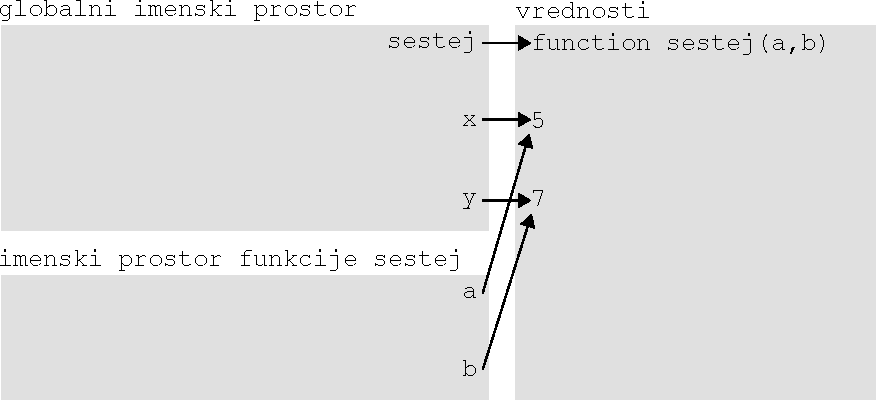
\includegraphics[width=\linewidth]{img/imenski_prostor_3.pdf}
    \caption{Ob klicu funkcije se ustvari njen lokalni imenski prostor znotraj katerega se dodatno ustvarijo plitve kopije vrednosti, s katerimi smo funkcijo poklicali.}
    \label{img:imenski_prostor_3}
\end{figure}
Vsa imena, ki jih bomo v nadaljevanju definirali znotraj funkcije, bodo ustvarjena v lokalnem imenskem prostoru funkcije. Ko naš program na primer izvede vrstico 2 (ta se je ob definiciji funkcije preskočila in se izvede šele ob njenem klicu), bo prišlo do situacije, kot jo prikazuje slika \ref{img:imenski_prostor_4}
\begin{figure}
    \centering
    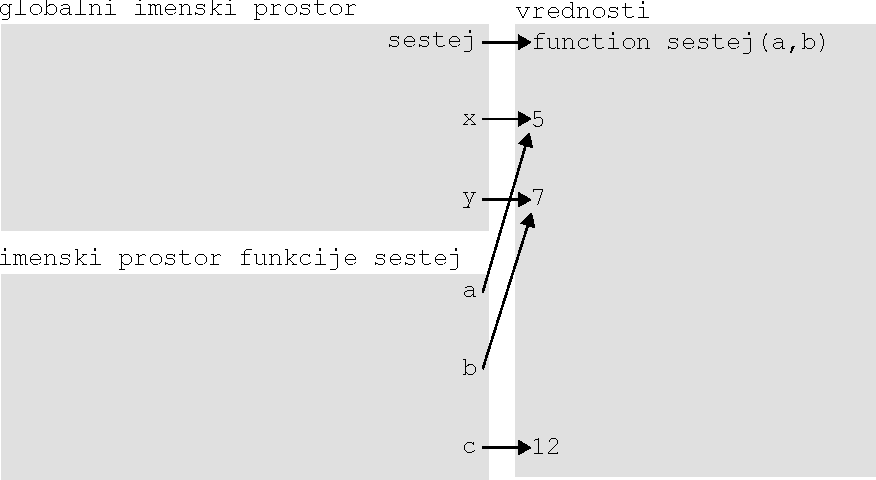
\includegraphics[width=\linewidth]{img/imenski_prostor_4.pdf}
    \caption{Vsa imena, ki jih definiramo znotraj funkcije, se ustvarijo zgolj v lokalnem imenskem prostoru te funkcije.}
    \label{img:imenski_prostor_4}
\end{figure}
Kaj pa bi se zgodilo, če bi znotraj funkcije definirali ime, ki obstaja že v globalnem imenskem prostoru. Nič posebnega. Spremenljivka s tem imenom bi se ustvarila v lokalnem imenskem prostoru funkcije in to na globalno spremenljivko ne bi vplivalo. Zgodilo bi se nekaj takega kot prikazuje slika \ref{img:imenski_prostor_5}.
\begin{figure}
    \centering
    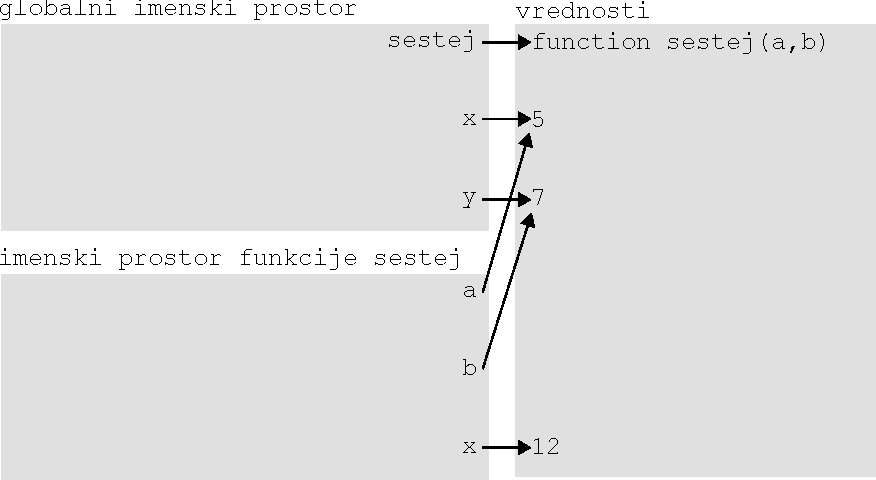
\includegraphics[width=\linewidth]{img/imenski_prostor_5.pdf}
    \caption{Znotraj funkcije lahko uporabljamo enaka imena spremenljivk kot izven funkcije in s tem ne vplivamo na globalne spremenljivke.}
    \label{img:imenski_prostor_5}
\end{figure}
Zakaj je tak način delovanja dober? Če bi morali znotraj funkcij paziti, da ne uporabljamo enakih imen, kot so že definirana izven funkcij, potem bi morali že vnaprej predvideti kakšna imena bodo pri programiranju uporabljali vsi bodoči uporabniki naših funkcij. Prav tako bi morali biti zelo pazljivi, ko bi obstoječe funkcije uporabljali mi. Vedeti bi morali katere spremenljivke za izpis nečesa na zaslon na primer uporablja funkcija \texttt{print}. Tem imenom bi se morali izogibati, kar pa bi bilo skrajno nerodno in nesmiselno.

Vprašanje, na katerega moramo še odgovoriti je, kaj se zgodi, ko se funkcija izvede do konca. V našem primeru se funkcija konča po izpisu vrednosti spremenljivke \texttt{c} (vrstica 3). Ko se funkcija konča, njenega lokalnega imenskega prostora ne potrebujemo več. Če bomo funkcijo še enkrat poklicali, bo Python pač ustvaril nov lokalen imenski prostor. Iz tega razloga, po končanju izvedbe funkcije, lokalni imenski prostor funkcije izgine. V našem konkretnem primeru torej imena \texttt{a}, \texttt{b} in \texttt{c} izginejo. Kaj pa vrednosti? Do vrednosti 12 ne moremo več dostopati preko nobene spremenljivke, zato se lahko izbriše tudi ta. Vrednosti 5 in 7 po drugi strani ostaneta, saj nanju še vedno kažeta imeni \texttt{x} in \texttt{y}. To prikazuje slika \ref{img:imenski_prostor_6}.
\begin{figure}
    \centering
    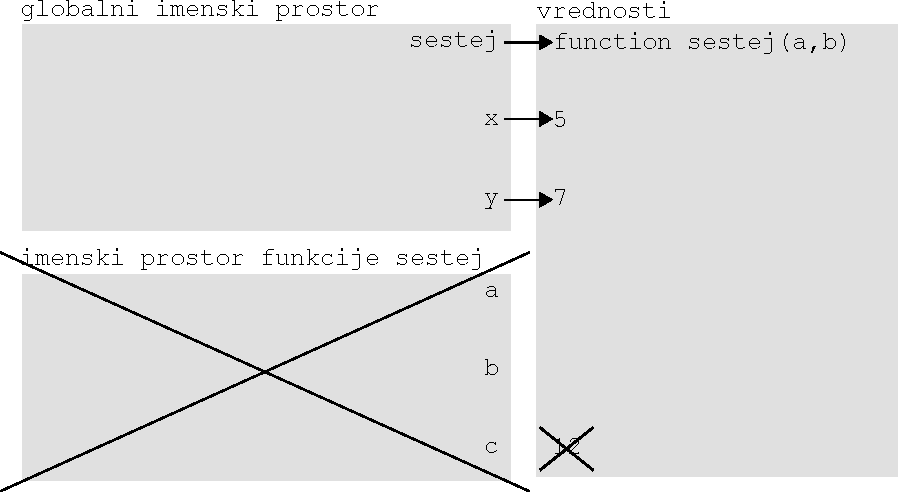
\includegraphics[width=\linewidth]{img/imenski_prostor_6.pdf}
    \caption{Po izvedbi klica funkcije, se njen imenski prostor izbriše.}
    \label{img:imenski_prostor_6}
\end{figure}

Iz globalnega imenskega prostora do lokalnih imenskih prostorov uporabljenih funkcij torej ne moremo dostopati, saj se po zaključku izvajanja funkcij (ko izvedba programa preide spet v globalni imenski prostor), lokalni imenski prostori izbrišejo. Kaj pa obratno? Iz lokalnega imenskega prostora funkcije, lahko dostopamo do globalnega (tudi zato se mu reče globalni), kar pomeni, da lahko dostopamo do vrednosti globalnih spremenljivk. Še pomembneje pa je to, da lahko iz lokalnega imenskega prostora funkcij, dostopamo do imen globalno definiranih funkcij. To pomeni, da lahko iz posamezne funkcije pokličemo druge funkcije (gnezdenje funkcij) ali pa tudi samo sebe. Slednjemu se reče \emph{rekurzija}, ampak pustimo to za kdaj drugič. 

Napišimo malo razširjen program, ki bo seštel vrednosti dveh seznamov. Pri tem si bomo pomagali z definicijo dveh funkcij.
\begin{lstlisting}[language=Python,numbers=left]
def sestej(a, b): # sestej in izpisi
    c = a + b
    print(c)

def sestej_seznama(a,b): # sestej istolezne elemente
    for i in range(len(a)):
        sestej(a[i], b[i])

sestej_seznama([1,2,3],[4,5,6]) # klic funkcije
\end{lstlisting}
Iz funkcije \texttt{sestej\_seznama} torej kličemo funkcijo \texttt{sestej}. Ali je to dovoljeno? Seveda. Imeni \texttt{sestej} in \texttt{sestej\_seznama} bomo po izvedbi vrstic 1 in 5 imeli v globalnem imenskem prostoru, kot prikazuje slika  \ref{img:imenski_prostor_7}.
\begin{figure}
    \centering
    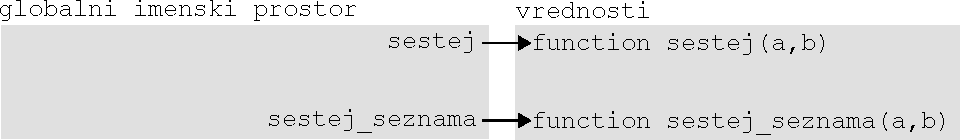
\includegraphics[width=\linewidth]{img/imenski_prostor_7.pdf}
    \caption{Imeni definiranih funkcij sta shranjeni v globalnem imenskem prostoru, zato jih lahko pokličemo od kjerkoli.}
    \label{img:imenski_prostor_7}
\end{figure}

Ker je globalni imenski prostor viden tudi iz lokalnih imenskih prostorov posameznih funkcij, jih lahko od tam tudi pokličemo. V sled temu je zgornji program popolnoma pravilen. 

Če program pogledamo podrobneje, lahko vidimo, da obe funkciji uporabljata enaka imena spremenljivk. Tudi to ne bo povzročalo nobenih težav, saj bo vsaka funkcija dobila svoj lasten lokalni imenski prostor. Ko bomo poklicali funkcijo \texttt{sestej\_seznama}, bo ta dobila lokalen imenski prostor. Ko bomo iz te funkcije poklicali funkcijo \texttt{sestej}, bo ta dobila svoj imenski prostor, ki se s prostorom funkcije \texttt{sestej\_seznama} ne bo prekrival. Lokalne imenske prostore si torej lahko predstavljamo kot ločene mehurčke, ki se med seboj ne prekrivajo. Stanje našega programa ob prvi izvedbi funkcije \texttt{sestej} do vključno vrstice 2 prikazuje slika \ref{img:imenski_prostor_8}.
\begin{figure}
    \centering
    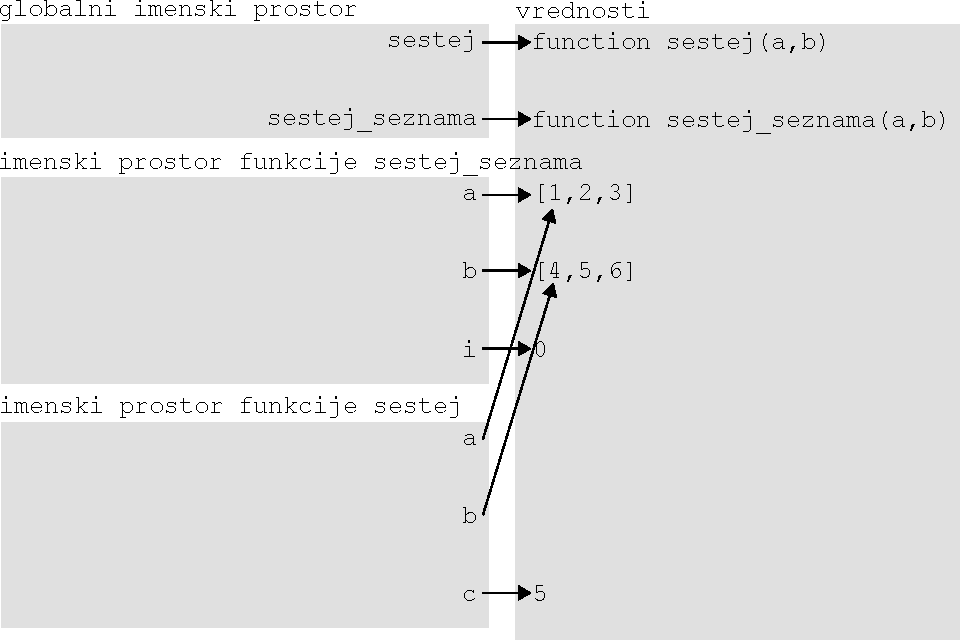
\includegraphics[width=\linewidth]{img/imenski_prostor_8.pdf}
    \caption{Lokalni imenski prostori funkcij so med seboj ločeni.}
    \label{img:imenski_prostor_8}
\end{figure}
Vprašanje za razmislek -- zakaj se znotraj funkcije \texttt{sestej} ne ustvarita novi vrednosti, na kateri bosta kazali imeni \texttt{a} in \texttt{b}?

\section{Vsaka funkcija vrača rezultat}
V splošnem pri programiranju ločimo dva tipa funkcij, in sicer tiste, ki nekaj uporabnega vrnejo in tiste, ki nekaj uporabnega naredijo (vrnejo pa nič). V določenih programskih jezikih ti dve skupini nosijo celo posebna imena in so tudi drugače definirane. Kaj pa v jeziku Python? V skupino funkcij, ki nekaj uporabnega vračajo bi lahko uvrstili npr. funkcijo \texttt{input}, ki prebere uporabnikov vnos in tega vrne kot podatkovni tip \texttt{str}. V skupino funkcijo, ki ne vračajo nič kaj preveč uporabnega, je pa uporabno tisto, kar naredijo, pa spada funkcija \texttt{print}. Dejstvo je, da v Pythonu vsaka funkcija nekaj vrne pa tudi, če to ni čisto nič uporabnega. Poglejmo si kaj vrne funkcija \texttt{print}. Kako? Rezultat funkcije \texttt{print} bomo shranili v spremenljivko in vrednost te spremenljivke izpisali.
\begin{lstlisting}[language=Python]
>>>a = print("testni izpis")
testni izpis
>>>print(a)
None
\end{lstlisting}
Kaj se torej skriva v rezultatu funkcije \texttt{print}? Dobesedno nič oziroma \texttt{None}. Funkcija nekaj vrne, in sicer vrne nič. Preverimo lahko tudi njegov podatkovni tip.
\begin{lstlisting}[language=Python]
>>>print(type(a))
<class 'NoneType'>
\end{lstlisting}
Nič oziroma \texttt{None} je torej poseben podatek, ki pripada podatkovnemu tipu nič oziroma \texttt{NoneType}. Ni sicer veliko, ampak nekaj pa je. Enak rezultat vračajo funkcije, ki smo jih definirali v prejšnjem razdelku. Lahko preverite sami.

Kaj pa če bi želeli, da naša funkcija vrne nekaj uporabnega? V tem primeru moramo od nje to eksplicitno zahtevati, in sicer s stavkom \texttt{return}.

Spremenimo funkcijo \texttt{sestej}, tako da bo vsoto dveh števil vračala in ne izpisovala.
\begin{lstlisting}[language=Python,numbers=left]
def sestej(a, b): # sestej in izpisi
    c = a + b
    return c
\end{lstlisting}
Z uporabo stavka \texttt{return} smo torej povedali, da želimo, da naša funkcija vrne vrednost spremenljivke \texttt{c}. Ali nismo tega naredili že prej? Ne. V prejšnji različici je funkcija vrednost spremenjivke \texttt{c} zgolj izpisovala. Ko se je funkcija končala, je njen lokalni imenski prostor izginil in z njim tudi vrednost spremenljivke \texttt{c}. Pogosto pa želimo rezultate funkcij uporabiti tudi v drugih delih naših programov (npr. ko uporabljamo funkcijo \texttt{input} želimo z uporabnikovim vnosom ponavadi nekaj uporabnega narediti in ga ne zgolj izpisati na zaslon). To lahko dosežemo s stavkom return. Kaj se zgodi, če funkcijo v našem programu zdaj še pokličemo. Razširimo program na sledeč način.
\begin{lstlisting}[language=Python,numbers=left]
def sestej(a, b): # sestej in vrni
    c = a + b
    return c
sestej(4,5)
\end{lstlisting}
Program tokrat ne izpiše ničesar. Zakaj ne? Ker tega od njega nismo nikjer zahtevali. Kaj torej naredi klic funkcije \texttt{sestej}. V konkretnem primeru nič uporabnega, saj izračuna vsoto števil 4 in 5, rezultat shrani v spremenljivko \texttt{c} in ko se funkcija zaključi, le-ta izgine, saj nanj ne kaže nobeno ime več. Kako pa bi lahko dobljeno vrednost uporabili še kje druge v našem programu? Podobno kot pri uporabi funkcije \texttt{input} -- tako, da bi rezultat funkcije priredili spremenljivki.
\begin{lstlisting}[language=Python,numbers=left]
def sestej(a, b): # sestej in vrni
    c = a + b
    return c
rezultat = sestej(4,5)
print(rezultat)
\end{lstlisting}
V zgornjem primeru bomo rezultat izpisali, lahko pa bi z njim naredili tudi karkoli drugega.

% zgled prastevila

Stavek \texttt{return} ima dvojno vlogo. Ob njegovem klicu funkcija vrne rezultat, poleg tega pa se njeno izvajanje prekine (podobno, kot če uporabimo stavek \texttt{break} v kombinaciji z zanko \texttt{while} ali \texttt{for}).

Povadimo zdaj to na iskanju praštevil. Najprej poskusimo napisati funkcijo, ki uporabniku informacijo o tem, ali število je praštevilo ali ne, zgolj izpiše.

\begin{zgled}
Napiši funkcijo, ki kot argument prejme celo število in izpiše, če je podano število praštevilo ali ne.
\end{zgled}

\begin{resitev} \  
\begin{lstlisting}[language=Python,numbers=left]
def prastevilo(stevilo):
    for i in range(2,stevilo): # razpon preiskovanja
        if stevilo % i == 0:
            print(stevilo, "ni prastevilo")
            break # dovolj je, da najdemo enega delitelja
    else: # ce se je zanka odvrtela do konca
        print(stevilo, "je prastevilo")   
\end{lstlisting}
\end{resitev}
Podoben program smo napisali že, ko smo se srečali z zanko \texttt{for}, tako da ga posebej ne bomo komentirali. Poskusimo zdaj program spremeniti, tako da ne bo ničesar izpisoval, ampak bo uporabniku podal povratno informacijo o tem, če je število praštevilo ali ne.
\begin{zgled}
Napiši funkcijo, ki kot argument prejme celo število in \textbf{vrne} vrednost \texttt{True}, če je to število praštevilo, sicer pa \textbf{vrne} vrednost \texttt{False}.
\end{zgled}
\begin{resitev} \  
\begin{lstlisting}[language=Python,numbers=left]
def prastevilo(stevilo):
    for i in range(2,stevilo): # razpon preiskovanja
        if stevilo % i == 0:
            return False # prekine funkcijo in vrne False
    return True # for se je odvrtel do konca
\end{lstlisting}
\end{resitev}
Ta rešitev je bistveno lepša in enostavnejša. Iz nje vidimo dodatno prednost stavka \texttt{return}, ki poleg vračanja rezultata prekine izvajanje funkcije. Ko smo v zanki \texttt{for} našli prvega delitelja, smo prekinili izvajanje funkcije in vrnili rezultat \texttt{False}. S prekinitvijo izvajanja funkcije se je prekinila tudi zanka, zato \texttt{break} ni več potreben. Če je program prišel do vrstice številka 5, zagotovo nismo našli nobenega delitelja, saj bi sicer funkcija že vrnila \texttt{False} in se nehala izvajati. Zato lahko v vrstici 5 brezpogojno vrnemo vrednost \texttt{True}. Tako tukaj ne potrebujemo niti stavka \texttt{if}.

Dodatna prednost te rešitve je tudi to, da lahko zdaj rezultat preverjanja uporabimo tudi kje drugje. Lahko na primer napišemo funkcijo, ki izpiše vsa praštevila v določenem razponu.
\begin{zgled}
Napiši funkcijo, ki kot argument prejme celo število in izpiše vsa praštevila do vključno podanega števila.
\end{zgled}
\begin{resitev} \  
\begin{lstlisting}[language=Python,numbers=left]
def prastevila(stevilo):
    for kandidat in range(2,stevilo+1): # kandidati
        if prastevilo(kandidat): # ali je prastevilo
            print(kandidat)
\end{lstlisting}
\end{resitev}
Rešitev je izjemno enostavna. Sprehodili smo se čez vse možne kandidate za praštevila in za vsakega preverili, če je praštevilo. Kako? Tako, da smo poklicali funkcijo, ki vrne \texttt{True}, če je podano število praštevilo. Klic te funkcije smo samo še vstavili v stavek \texttt{if}, ki je izpisal število v primeru izpolnjenosti pogoja.

\section{Izbirni argumenti}
V določenih primerih želimo, da imajo določeni argumenti funkcije svoje vrednosti že vnaprej določene, razen v primeru, da uporabnik želi za te argumente uporabiti druge vrednosti. Če torej uporabnik vrednosti argumentov ne bo podal, bodo uporabljene njihove privzete vrednosti. V nasprotnem primeru bodo uporabljene uporabnikove vrednosti. Tak primer uporabe funkcij smo srečali že pri funkciji \texttt{print}, ki ima kar nekaj izbirnih argumentov. Privzeto gre funkcija \texttt{print} po vsakem klicu v novo vrstico (argument \texttt{end} je privzeto enak znaku za novo vrstico -- \texttt{\\n}), v primeru več podanih vrednosti pa te izpišejo tako, da se med njih vrine presledke (argument \texttt{sep} je privzeto enak presledku). Njune privzete vrednosti lahko povozimo, tako da jih specificiramo ob klicu, npr. kot
\begin{lstlisting}[language=Python]
>>> print(1,2,3,sep='+',end=' ')
1+2+3
\end{lstlisting}
Podobno lahko specificiramo izbirne argumente in njihove vrednosti pri definiciji svojih funkcij. 
\begin{lstlisting}[language=Python]
def ime_funkcije(arg1, arg2,..., opc1=v1, opc2=v2,...):
\end{lstlisting}
Paziti moramo samo na to, da so tisti argumenti, ki nimajo privzetih vrednosti vedno podani pred tistimi, ki privzete vrednosti imajo.

Povadimo to na malo bolj splošnem Fibonaccijevem zaporedju. Najprej poskusimo brez uporabe opcijskih argumentov.
\begin{zgled}
Napiši funkcijo, ki vrne Fibonaccijevo zaporedje števil, pri čemer naj uporabik poda dolžino zaporedja in prvi dve števili v zaporedju.
\end{zgled}
\begin{resitev} \  
\begin{lstlisting}[language=Python,numbers=left]
def fibonacci(n, a, b):
    if n == 1:
        return [a]
    f = [a,b]
    for i in range(3,n+1):
        f.append(f[-1]+f[-2])
    return f
\end{lstlisting}
\end{resitev}
V primeru, da uporabnik želi imeti zaporedje dolžine 1, funkcija vrne zaporedje z enim elementom, in sicer \texttt{a}. V nasprotnem primeru naredi začetno zaporedje z elementoma \texttt{a} in \texttt{b} in potem v zanki doda ustrezno število dodatnih elementov, ki vsakič predstavljajo vsoto zadnjih dveh elementov zaporedja. S to rešitvijo sicer ni nič narobe, je pa dejstvo to, da si kot Fibonaccijevo zaporedje ponavadi predstavljamo zaporedje števil, ki se začne z vrednostima 1, 1. Smiselno bi torej bilo, da se privzeto naše zaporedje začne s števili 1, 1, razen če uporabnik tega ne specificira drugače. 
\begin{zgled}
Napiši funkcijo, vrne Fibonaccijevo zaporedje števil, pri čemer naj uporabik poda dolžino zaporedja. Uporabnik lahko poda tudi prvi dve števili v zaporedju, ki sta privzeto enaki 1.
\end{zgled}
\begin{resitev} \  
\begin{lstlisting}[language=Python,numbers=left]
def fibonacci(n, a=1, b=1):
    if n == 1:
        return [a]
    f = [a,b]
    for i in range(3,n+1):
        f.append(f[-1]+f[-2])
    return f
\end{lstlisting}
\end{resitev}
Zgornjo funkcijo lahko torej pokličemo tudi tako, da podamo samo dolžino zaporedja. V tem primeru bosta prvi dve števili v zaporedju enaki 1, 1. V primeru, da jo bomo poklicali tako, da podamo še vrednosti za argumenta \texttt{a} in \texttt{b} pa bosta za začetna elementa uporabljeni ti vrednosti.
\chapter{Uporaba in pisanje modulov}

\section{Kaj so moduli?}

Moduli predstavljajo Pythonove datoteke, ki vsebujejo implementacijo določenih funkcij, spremenljivk in razredov \angl{classes}. Module lahko vključimo v svoje programe in na ta način razširimo osnovne funkcionalnosti jezika Python. Primeri že vgrajenih modulov, ki jih ni potrebno posebej namestiti, so modul \texttt{math}, v katerem so definirane določene matematične funkcije in konstante, modul \texttt{time} za vračanje podatkov o času in tvorjenje zakasnitev ter modul \texttt{random} za delo s (psevdo)naključnimi števili.

\section{Uporaba modulov}

Module lahko v svoje programe vključimo na različne načine, v vseh primerih pa uporabljamo rezervirano besedo \texttt{import}. Če želimo npr. v naš program uvoziti celoten modul \texttt{math}, lahko to naredimo s sledečo vrstico:
\begin{lstlisting}[language=Python]
import math
\end{lstlisting}
oziroma v splošnem
\begin{lstlisting}[language=Python]
import ime_modula
\end{lstlisting}
Najprej lahko preverimo kaj uvožen modul dejansko ponuja. Če je pisec modula bil priden in napisal tudi dokumentacijo, bomo za to lahko uporabili funkcijo \texttt{help}
\begin{lstlisting}[language=Python]
help(ime_modula)
\end{lstlisting}
Funkcija nam bo izpisala nekaj osnovnih informacij o modulu, tako da bo uporaba lažja. Seveda pa lahko informacije o modulu poiščemo tudi na internetu, ki pa včasih ni na voljo (npr. v času pisanja kolokvijev in izpitov), zato se je dobro navaditi tudi uporabe zgoraj omenjene funkcije.

Če bi zdaj želeli dostopati do posamezen funkcije, ki je v uvoženem modulu definirana, bi to naredili na sledeč način
\begin{lstlisting}[language=Python]
ime_modula.ime_funkcije(argumenti)
\end{lstlisting}
Če bi npr. želeli izračunati sinus števila shranjenega v spremenljivki \texttt{x} in rezultat shraniti v spremenljivko \texttt{y}, bi za to uporabil funkcijo \texttt{sin}, ki je vsebovana v modulu \texttt{math}. Poklicali bi jo takole
\begin{lstlisting}[language=Python]
y=math.sin(x)
\end{lstlisting}

Včasih imajo moduli zelo dolga in težko berljiva imena. Če želimo modul uvoziti pod drugačnim imenom (lahko bi rekli psevdonimom), uvoz dopolnimo z \texttt{as} stavkom:
\begin{lstlisting}[language=Python]
import dolgo_ime_modula as psevdonim
\end{lstlisting}
Tako lahko pri klicanju funkcij (ali pa česarkoli že) modula podajamo le kratko ime modula. V prejšnjem primeru bi kodo lahko spremenili na sledeč način:
\begin{lstlisting}[language=Python]
import math as m
y=m.sin(x)
\end{lstlisting}

V določenih primerih pa želimo iz modula uvoziti le določeno funkcijo (spremenljivko, razred). Takrat lahko uporabimo rezervirano besedo \texttt{from}, in sicer takole
\begin{lstlisting}[language=Python]
from ime_modula import ime_funkcije
\end{lstlisting}
S takim načinom uvažanja smo uvozili le tisto kar potrebujemo, poleg tega pa zdaj pri klicu funkcije imena modula ni potrebno več podajati. Primer sinusa bi se spremenil v sledečo kodo
\begin{lstlisting}[language=Python]
from math import sin
y=sin(x)
\end{lstlisting}
Zdaj smo iz modula uvozili zgolj funkcijo \texttt{sin} -- če bi želeli imeti še kakšno drugo funkcijo, npr. kosinus, bi jo morali uvoziti ločeno oziroma hkrati s funkcijo \texttt{sin}. To bi naredili takole:
\begin{lstlisting}[language=Python]
from math import sin,cos
\end{lstlisting}
Lahko pa naredimo še nekaj, kar ponavadi ni priporočljivo. Uvozimo lahko vse, kar je v modulu definirano, in sicer namesto imena funkcije podamo \texttt{*}, ki se v računalništvu velikokrat uporablja kot simbol za \emph{vse}. Rekli bomo torej \emph{iz modula uvozi vse}:
\begin{lstlisting}[language=Python]
from ime_modula import *
\end{lstlisting}
V primeru modula \texttt{math} bomo zapisali takole:
\begin{lstlisting}[language=Python]
from math import *
\end{lstlisting}
Zakaj tak način uvažanja ni priporočljiv? Vse funkcije, spremenljivke in razrede modula smo zdaj dobili v naš globalni imenski prostor. Pri tem je velika verjetnost, da smo si s tem povozili kakšno od spremenljivk, ki jo tam že uporabljamo in ima enako ime kot kakšna izmed funkcij ali spremenljivk definiranih v modulu. Zato se takemu način uvažanja modulov izogibamo.

\section{Definicija in uporaba lastnih modulov}
Vsi programi, ki smo jih do zdaj napisali, predstavljajo module, ki jih lahko uvozimo v druge programe. To pomeni, da pri reševanju nekega (bolj kompleksnega) problema ni potrebno vse kode napisati v isti datoteki, ampak lahko datoteko razdelimo po smiselnih modulih, pri čemer lahko funkcije prvega modula uporabljamo v drugem in obratno. Pri tem lahko uporabimo kodo opisano v prejšnjem razdelku. Paziti moramo le na to, da se modul, ki ga uvažamo nahaja v isti mapi kot modul, v katerega kodo uvažamo. V nasprotnem primeru moramo pri uvažanju modula do drugega modula podati še pot do njega. Če se modul, ki ga želimo uvoziti, npr. nahaja v podmapi mapi \texttt{podmapa}, ga bomo uvozili na sledeč način:
\begin{lstlisting}[language=Python]
import podmapa.ime_modula
\end{lstlisting}
Če v tem primeru ne želimo, da modul vsakič posebej kličemo z imenom \texttt{podmapa.ime\_modula}, ga je smiselno uvoziti pod krajšim imenom takole
\begin{lstlisting}[language=Python]
import podmapa.ime_modula as ime_modula
\end{lstlisting}
Mogoče se sprašujete zakaj poti ni bilo potrebno podajati pri uvažanju modula \texttt{math}. Dejstvo je, da so določeni moduli v Python že vgrajeni, sicer pa Python module, poleg v trenutni delovni mapi, išče tudi v mapi \texttt{lib$\backslash$site-packages}, kamor se shranijo namestitve vseh modulov, ki jih bomo v prihodnosti potencialno še namestili.

\section{Nameščanje novih modulov}
Na spletu obstaja veliko modulov, ki so jih razvili programerji pred nami. Te lahko uporabimo, kadar želimo pri reševanju določenega problema uporabiti višjenivojske sestavine. Če želimo npr. narisati graf povprečne mesečne plače v Sloveniji, nam ni potrebno študirati, kako se lotili kakršnegakoli risanja v jeziku Python, ampak enostavno uporabimo paket (paket ni nič drugega kot zbirka modulov) \texttt{matplotlib} in njegove funkcije za risanje grafov. Problem, s katerim se srečamo, je, da tovrstni paketi v osnovni različici Pythona še niso nameščeni (razen, če si nismo namestili distribucije Anaconda \footnote{Anaconda je distribucija Pythona za znanstveno računanje, ki ima nameščenih že večino paketov, ki jih za tako računanje potrebujemo. Dostopna je na povezavi \url{https://www.anaconda.com/}.}) Pred uporabo jih moramo torej namestiti. Problem nameščanja tovrstnih paketov je, poleg včasih mukotrpnega procesa iskanja ustreznih namestitvenih datotek in ročne namestitive, tudi v tem, da za svoje delovanje večina paketov uporablja druge pakete, ti paketi spet druge in tako naprej. Temu rečemo odvisnost med paketi \angl{package dependency}. Da pa se s tem običajnemu uporabniku Pythona ni potrebno ukvarjati, Python okolje vsebuje orodje \texttt{pip} \angl{pip installs packages}, ki preko repozitorija PyPI \angl{Python package index} poišče in namesti ustrezne pakete avtomatsko. Nameščen je že skuppaj z osnovno distribucijo Pythona. Vse kar poleg tega potrebujemo je še internetna povezava in ime paketa, ki ga želimo namestiti. Orodje \texttt{pip} bomo pognali iz sistemske ukazne vrstice (v operacijskem sistemu Widnows jo zaženemo tako, da v start meni vpišemo \texttt{cmd}). V primeru, da smo ob namestitivi Pythona obkljukali opcijo \emph{Add Python to path}, lahko orodje \texttt{pip} poženemo iz poljubne lokacije. V nasprotnem primeru se moramo premakniti v mapo, kjer \texttt{pip} nameščen (podmapa \texttt{Scripts} mape, kjer je nameščen Python). Paket z imenom \texttt{ime\_paketa}  zdaj namestimo s sledečim ukazom
\begin{lstlisting}[language=bash]
>>> pip install ime_paketa
\end{lstlisting}
in \texttt{pip} bo poskrbel za vse ostalo.

%\section{Primeri uporabe modulov}

%\subsection{Modul \texttt{math}}

%\begin{lstlisting}[language=Python]
%help(math)
%\end{lstlisting}




\chapter{Spremenljivost podatkovnih tipov in terke}

\section{Kaj je spremenljivost?}

Določeni podatkovni tipi v Pythonu so spremenljivi \angl{mutable}, določeni pa ne. Kaj to pomeni? Če je nek podatek nespremenljiv \angl{immutable}, to pomeni, da ga po tistem, ko je enkrat ustvarjen, ne moremo več spreminjati. Lahko pa naredimo nov podatek, ki odraža spremembo, ki jo želimo nad podatkom narediti. Primeri nespremenljivih podatkovnih tipov so števila tipa \texttt{int} in \texttt{float}, niz oziroma \texttt{str} in \texttt{bool} (spremenljivost osnovnih podatkovnih tipov v jeziku Python prikazuje tabela \ref{tab:spremenljivost}). To so torej skoraj vsi podatkovni tipi, ki smo jih do sedaj spoznali. Če je določen podatek spremenljiv, potem ga lahko spreminjamo tudi kasneje. Primer spremenljivega podatkovnega tipa je seznam oziroma \texttt{list}. Spremenljivost podatkovnih tipov na videz izgleda kot nekaj, s čimer se nam pri osnovah programiranja niti ne bi bilo potrebno ukvarjati. Žal pa ima veliko posledic, ki jih brez razumevanja spremenljivosti težko razumemo, zato je smiselno, da si celoten koncept podrobneje pogledamo. 
\begin{table}
    \caption{Spremenljivost osnovnih podatkovnih tipov v jeziku Python}
    \label{tab:spremenljivost}
    \centering
    \begin{tabular}{c|c|c}
    podatkovni tip & opis & spremenljiv  \\
    \hline
    \texttt{bool}& \textit{boolean} (\texttt{True, False}) & Ne \\
    \texttt{int}& \textit{integer} (celo število) & Ne \\
    \texttt{float}& \textit{floating-point} (decimalno število) & Ne \\
    \texttt{str}& \textit{string} (niz) & Ne \\
    \texttt{list}& \textit{list} (seznam) & Da \\
    \texttt{tuple}& \textit{tuple} (terka) & Ne \\
    \texttt{dict}& \textit{dictionary} (slovar) & Da \\
    \texttt{set}& \textit{set} (množica) & Da \\
    \texttt{frozenset}& \textit{frozenset} (nespremenljiva množica) & Ne \\
    \end{tabular}
\end{table}

\section{Kaj se zgodi ob prirejanju spremenljivk?}
Kaj se zgodi, ko spremenljivki priredimo neko vrednost že vemo. V imenskem prostoru, kjer spremenljivko definiramo, se pojavijo imena, ki smo jih dodelili spremenljivkam, v pomnilniku pa se ustvarijo vrednosti, na katere ta imena kažejo. Zapoerdje prireditvenih stavkov
\begin{lstlisting}[language=Python]
>>> i = 1
>>> niz = 'ABC'
>>> seznam = [1,2,3]
\end{lstlisting}
lahko ponazorimo s sliko \ref{img:spremenljivost}.
\begin{figure}
    \centering
    
\includegraphics[width=\linewidth]{img/spremenljivost.pdf}
    \caption{Ob prireditvi se imenu spremenljivke priredi podana vrednost.}
    \label{img:spremenljivost}
\end{figure}
Kaj pa se zgodi, če spremenljivko priredimo drugi spremenljivki, na primer takole:
\begin{lstlisting}[language=Python]
>>> i = 1
>>> j = i
>>> niz1 = 'ABC'
>>> niz2 = niz1
>>> seznam1 = [1,2,3]
>>> seznam2 = seznam1
\end{lstlisting}
Nekaj podobnega smo srečali že pri klicu funkcije. Spomnimo se, da se v Pythonu v takem primeru naredi t.i. \textit{plitva kopija} spremenljivke. To pomeni, da vrednost v pomnilniku dobi novo ime. Do dejanskega (\textit{globokega}) kopiranja vrednosti v tem primeru ne pride. To lahko ponazorimo s sliko \ref{img:spremenljivost_2}.
\begin{figure}
    \centering
    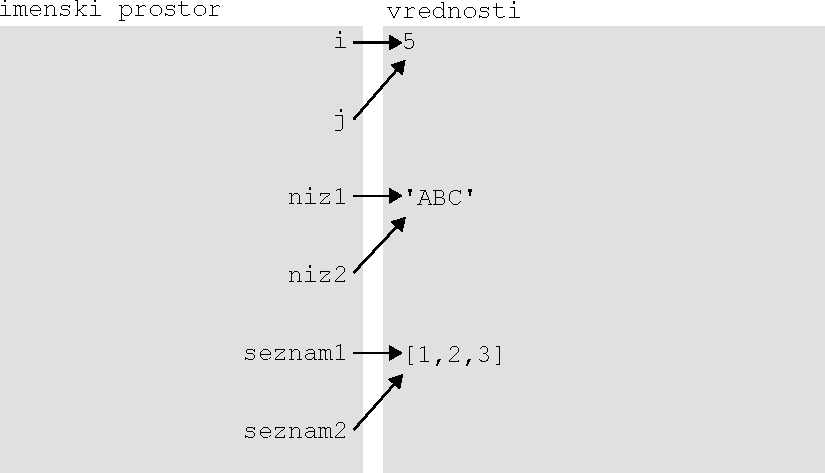
\includegraphics[width=\linewidth]{img/spremenljivost_2.pdf}
    \caption{Ob prireditvi spremenljivke drugi spremenljivki se ustvari plitva kopija spremenljivke.}
    \label{img:spremenljivost_2}
\end{figure}
Na tak način je delovanje tako s časovnega stališča (hitrost) kot tudi s prostorskega stališča (poraba pomnilnika) bolj varčno. 

\section{Kaj se zgodi ob spreminjanju vrednosti spremenljivk?}
Kaj pa se zgodi, če vrednost nove (ali pa stare) spremenljivke spremenimo? Vse skupaj zavisi od tega ali je podatek, ki ga spreminjamo spremenljiv ali ne. Spomnimo se. Spremenljiv podatek lahko spreminjamo, ko pa pokusimo spremeniti nespremenljiv podatek, se ustvari njegova kopija (globoka), ki odraža narejeno spremembo. Če npr. uporabimo operator \texttt{+=}, bo v primeru spremenljivega podatka spremenjen obstoječ podatek, v primeru nespremenljivega podatka pa bo ustvarjen nov podatek, ki bo odražal narejeno spremembno. 

Kaj pa se zgodi v primeru, da na podatek kaže več imen, kot v scenariju zgoraj. Ali se bo po izvedbi spodnje kode sprememba odražala tudi preko drugih imen podatka? Poglejmo si spodnjo kodo.
\begin{lstlisting}[language=Python]
>>> i = 1
>>> j = i
>>> j += 1
>>> niz1 = 'ABC'
>>> niz2 = niz1
>>> niz2 += 'D'
>>> seznam1 = [1,2,3]
>>> seznam2 = seznam1
>>> seznam2 += [4]
\end{lstlisting}
Zanima nas ali se po spreminjanju spremenljivk \texttt{j}, \texttt{niz2} in \texttt{seznam2} spremembe odražajo tudi na spremenljivkah \texttt{i}, \textbf{niz1} in \texttt{seznam1}. Odgovor ni enostvane da ali ne. Odgovor je namreč odvisen od spremenljivosti podatka, ki ga spreminjamo. Situacijo po spreminjanju podatka z operatorjem \texttt{+=} prikazuje slika \ref{img:spremenljivost_3}.
\begin{figure}
    \centering
    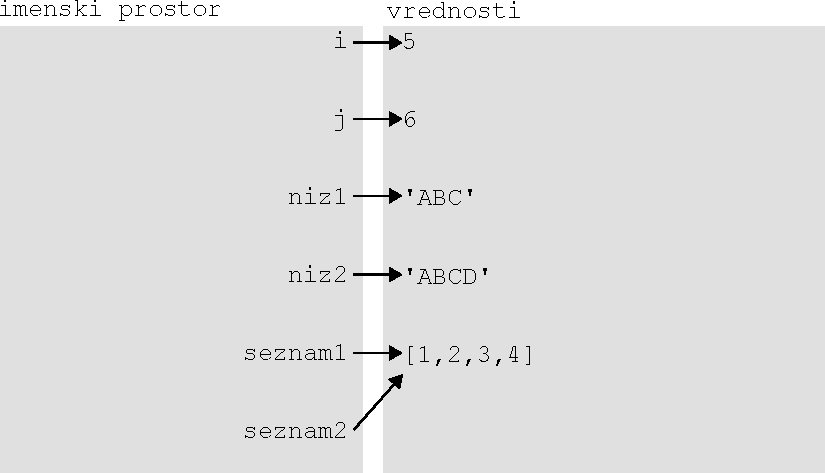
\includegraphics[width=\linewidth]{img/spremenljivost_3.pdf}
    \caption{Ob spreminjanju spremenljivih podatkov se spremenijo vse plitve kopije podatka.}
    \label{img:spremenljivost_3}
\end{figure}
V primeru, da je podatek spremenljiv, se torej sprememba odraža na vseh spremenljivkah, ki predstavljajo plitve kopije tega podatka. S tem ko v zgornjem zgledu spreminjamo spremenljivko \texttt{seznam2}, spreminjamo tudi spremenljivko \texttt{seznam1}. Po drugi strani spreminjanje spremenljivk \texttt{j} in \texttt{niz2} ustvari globoko kopijo spremenljivk \texttt{j} in \texttt{niz2}, ki odraža narejeno spremembo. Globoka kopija predstavlja nov podatek, tj. podatek ki se razlikuje od tistega, na katerega kažeta imeni \texttt{i} in \texttt{niz1}. Posledica tega je, da spreminjanje vrednosti spremenljivk \texttt{j} in \texttt{niz2} na vrednostih spremenljivk \texttt{i} in \texttt{niz1} ne vplivajo, saj pripadajo nespremenljivim podatkovnim tipom.

\section{Ali funkcije spreminjajo vrednosti svojim argumentom?}
Spomnimo se, da se ob klicu funkcije ustvari lokalni imenski prostor funkcije. V lokalnem imenskem prostoru se ob klicu spremenljivkam, ki nastopajo kot argumenti funkcije, priredijo vrednosti, s katerimi smo funkcijo poklicali. V primeru, da smo funkcijo poklicali z globalnimi spremenljivkami, se argumentom funkcije priredi plitva kopija teh spremenljivk. Vprašanje pa je ali se bodo ob spreminjanju argumentov funkcije spremembe odražale tudi izven funkcije, torej po tem, ko se bo funkcija že končala. Vprašanje lahko ponazorimo s spodnjim zgledom.

\begin{zgled}
Kakšna je vrednost spremenljivk \texttt{st1}, \texttt{niz1} in \texttt{seznam1} po izvedbi spodnje kode in kakšen bo izpis programa?
\begin{lstlisting}[language=Python,numbers=left]
def spremeni(a, b):
    a += b

i = 1
j = 2
spremeni(i,j)
print(i)

niz1 = "ABC"
niz2 = "D"
spremeni(niz1,niz2)
print(niz1)

seznam1 = [1,2,3]
seznam2 = [4,5,6]
spremeni(seznam1,seznam2)
print(seznam1)
\end{lstlisting}
\end{zgled}

\begin{resitev}
Ob klicu funkcije spremenljivki, s katerima funkcijo pokličemo, dobita plitvi kopiji z imeni \texttt{a} in \texttt{b} v lokalnem imenskem prostoru funkcije. Znotraj funkcije plitvo kopijo z imenom \texttt{a} spreminjamo. V primeru, da je spremenljivka spremenljivega podatkovnega tipa (npr. seznam) se spreminja obstoječ podatek, na katerega kaže tudi globalna spremenljivka, kar pomeni, da se bo sprememba odražala tudi izven funkcije. V primeru, da je spremenljivka nespremenljivega podatkovnega tipa, se ustvari globoka kopija podatka, ki bo odražala narejeno spremembo. Spremeni se torej zgolj spremenljivka, ki je definirana znotraj funkcije, ta sprememba pa izven funkcije ne bo vidna. 

Spremenljivki \texttt{i} in \texttt{niz1} se torej po klicu funkcije ne bosta spremenili, spremenljivka \texttt{seznam1} pa se bo spremenila. Po izvedbi programa bo izpis sledeč:

\begin{lstlisting}[language=Python]
1 # nespremenjena vrednost
ABC # nespremenjena vrednost
[1,2,3,4,5,6] # spremenjena vrednost
\end{lstlisting}

\end{resitev}

Funkcije torej lahko spreminjajo vrednosti svojim argumentom, tako da so spremembe vidne tudi izven funkcij, ampak samo v primeru, ko so podani argumenti spremenljivega podatkovnega tipa. 



\section{Terke}

Zdaj, ko vemo, kaj je to spremenljivost, lahko razložimo tudi, kaj so terke \angl{tuples}. Terka oziroma \texttt{tuple} predstavlja sekvenčen podatkovni tip, ki je nespremenljiv. Ker terke zelo spominjajo na sezname, bi jim lahko rekli tudi nespremenljivi seznami. Načeloma bi lahko pri programiranju shajali tudi brez njih (tako kot bi lahko shajali tudi brez zanke \texttt{for}), ampak njihova uporaba v veliko primerih naredi naše programe lepše in boljše (tako kot uporaba zanke \texttt{for}).

\section{Uporaba terk}

Terko definiramo z navadnimi oklepaji, tj. \texttt{(} in \texttt{)}, znotraj katerih naštejemo elemente. Terko treh elementov, bi lahko definirali na primer takole:
\begin{lstlisting}[language=Python]
>>> terka=("Janez", 1.8, 75)
\end{lstlisting}
Za terko je pa mogoče bolj kot oklepaji bistveno naštevanje elementov, zato bi tudi, če bi oklepaje izpustili, dobili terko. Takole:
\begin{lstlisting}[language=Python]
>>> terka="Janez", 1.8, 75
>>> terka
("Janez", 1.8, 75)
>>> type(terka)
<class 'tuple'>
\end{lstlisting}
Python je ob naštevanju elementov z vejicami ugotovil, da želimo imeti terko in jo naredil. Python ima nekoliko težav, ko želimo narediti terko dolžine 1, saj si v tem primeru oklepaje razlaga kot operator, ki določa prioriteto. V primeru, da znotraj oklepajev damo zgolj eno npr. celo število, bomo torej dobili podatek, ki pripada podatkovnemu tipu \texttt{int} in ne \texttt{tuple}:
\begin{lstlisting}[language=Python]
>>> terka=(1)
>>> terka
1
>>> type(terka)
<class 'int'>
\end{lstlisting}
Že prej smo omenili to, da je bistvena lasntnost terk naštevanje elementov, ki jih ločimo z vejicami. Kako v primeru enega elementa povemo, da gre za naštevanje? Tako, da za njim napišemo vejico:
\texttt{tuple}:
\begin{lstlisting}[language=Python]
>>> terka=(1,)
>>> terka
(1,)
>>> type(terka)
<class 'tuple'>
\end{lstlisting}
Gre pa seveda tudi brez oklepajev:
\texttt{tuple}:
\begin{lstlisting}[language=Python]
>>> terka=1,
>>> terka
(1,)
>>> type(terka)
<class 'tuple'>
\end{lstlisting}

Kaj lahko s terkami počnemo? Podobno kot sezname lahko elemente terke indeksiramo, lahko delamo rezine, lahko preverjamo vsebovanost elementov, z zanko \texttt{for} se lahko čez elemente terke sprehajamo itd. Z njimi lahko delamo torej skoraj vse, kar smo delali s seznami. Skoraj vse? Ker so terke nespremenljive, jih seveda ne moremo spreminjati, tako kot lahko spreminjamo sezname. Poskusimo:
\begin{lstlisting}[language=Python]
>>> terka = ("Janez", 1.8, 75)
>>> terka[0] = "Marko"
Traceback (most recent call last):
  File "<pyshell#6>", line 1, in <module>
    terka[0] = "Marko"
TypeError: 'tuple' object does not support item assignment
\end{lstlisting}
Očitno res ne gre. Seveda ne, saj so nespremenljive. Zakaj bi terke potem sploh uporabljali? Nekaj primerov, pri katerih je uporaba terk smiselna, je podanih v nadaljevanju poglavja.

\section{Seznami terk in razpakiranje elementov terk}

Nenapisano pravilo (ki ga seveda lahko kršimo) je, da v sezname shranjujemo homogene podatke, torej podatke, ki se nanašajo npr. na isto spremenljivko. To pomeni, da vsak element seznama obravnavamo na enak način, saj se nanaša na isto količino. Terke se pogosto uporabljajo za shranjevanje heterogenih podatkov, tj. podatkov različnih tipov, ki pa pripadajo isti entiteti, kot je npr. oseba ali meritev. Če si torej želimo pri določeni entiteti zabeležiti več podatkov, lahko uporabimo seznam terk. Na primer, če imamo vzorec oseb, pri čemer za vsako osebo beležimo ime, višino in težo, potem lahko uporabimo seznam terk, pri čemer vsaka izmed terk vsebuje ime, višino in težo dotične osebe. Primer takega seznama bi bil
\begin{lstlisting}[language=Python]
meritve = [("Janez", 1.8, 75),
           ("Ana", 1.65, 60), 
           ("Nika", 1.66, 55)]
\end{lstlisting}
Elementi seznama so torej homogeni, kar pomeni, da bomo vsakega obravavali enako. Elementi seznama so namreč terke, ki imajo vsakič enako obliko. Na 0-tem indeksu je shranjeno ime osebe, na indeksu 1 višina v metrih in na indeksu 2 teža osebe v kilogramih. Elementi posamezne terke pa očitno pripadajo različnim spremenljivkam.

Tak način predstavitve podatkov bomo srečali velikokrat. Kako pa lahko tako shranjene podatke uporabimo pri nadaljnji analizi. Na primer pri izračunu in izpisu indeksa telesnih mas posamezne osebe v seznamu. Tako, da se čez seznam sprehodimo z zanko \texttt{for} in v vsaki iteraciji zanke tekočo terko \emph{razpakiramo} in tako pridemo do konkretnih vrednosti. To lahko naredimo na sledeč način: 
\begin{lstlisting}[language=Python]
for meritev in meritve:
    ime = meritev[0]
    visina = meritev[1]
    teza = meritev[2]
    itm = teza/visina**2
    print("ITM osebe", ime, "je", itm)
\end{lstlisting}
Do posameznih elementov terke smo torej prišli z njihovim indeksiranjem. Terke pa lahko razpakiramo veliko hitreje, in sicer tako, da terko priredimo drugi terki, ki vsebuje imena spremenljivk, v katere želimo vrednosti shraniti oziroma razpakirati. Takole:
\begin{lstlisting}[language=Python]
(spremenljivka1, spremenljivka2,...) = terka
\end{lstlisting}
Paziti moramo le na to, da terka na levi strani vsebuje enako število elementov kot terka na desni strani prireditvenega stavka. Kaj smo v zgornjem stavku pravzaprav naredili? Naredili smo terko spremenljivk, ki smo ji priredili terko na desni strani. Ker terki spremenljivk nismo dali nobenega imena, je v imenski prostor nismo shranili in zato tudi ni shranjena nikjer v pomnilniku. So pa v pomnilniku ostale spremenljivke, v katere smo razpakirali terko na desni. Kot smo videli že zgoraj pa lahko oklepaje pri definiciji tudi izpustimo. Torej lahko napišemo tudi nekaj takega
\begin{lstlisting}[language=Python]
spremenljivka1, spremenljivka2,... = terka
\end{lstlisting}
Mimogrede, tako razpakiranje elementov bi delovalo tudi, če bi imeli na desni strani prireditvnega stavka seznam.

Tak način razpakiranja elementov lahko uporabimo v našem zgledu z računanjem indeksa telesnih mas, s čimer se koda občutna skrajša:
\begin{lstlisting}[language=Python]
for meritev in meritve:
    ime, visina, teza = meritev
    itm = teza/visina**2
    print("ITM osebe", ime, "je", itm)
\end{lstlisting}
Kodo lahko še dodatno skrajšamo, če razpakiranje naredimo kar v glavi zanke \texttt{for}:
\begin{lstlisting}[language=Python]
for ime, visina, teza in meritve:
    itm = teza/visina**2
    print("ITM osebe", ime, "je", itm)
\end{lstlisting}

\section{Pakiranje seznamov v sezname terk}
Seznami terk, kot smo jih srečali zgoraj, torej predstavljajo lep način zapisovanja podatkov, ko želimo pri posamezni entiteti imeti več podatkov. Dejstvo pa je, da velikokrat podatkov ne dobimo v taki obliki, ampak dobimo za vsako količino svoj seznam. Pri tem so seznami med seboj poravnani, kar pomeni, da istoležni elementi v vseh seznamih pripadajo isti entiteti. Elementi na indeksu 0 torej pripadajo entiteti 0, elementi na indeksu 1 entiteti 1 itd. V primeru imen, višin in tež, bi torej imeli tri sezname v obliki 
\begin{lstlisting}[language=Python]
imena = ["Janez", "Ana", "Nika"]
visine = [1.8, 1.65, 1.66]
teze = [75, 60, 55]
\end{lstlisting}
Elementi vseh treh seznamov torej na indeksu 0 pripadajo Janezu, na indeksu 1 Ani in na indeksu 2 Niki. Kaj imajo ti seznami skupnega? Indekse! Čez take podatke bi se torej lahko sprehodili tako, da se sprehajamo po indeksih in ne direktno po elementih. Naredimo torej sprehod z znako \texttt{for} od indeksa 0 do dolžine seznama - 1. Dolžine katerega seznama? Ni važno, saj so vsi enko dolgi (oziroma vsaj smiselno bi bilo, da so). To bi lahko naredili takole:  
\begin{lstlisting}[language=Python]
for i in range(len(imena)):
    ime = imena[i]
    visina = visine[i]
    teza = teze[i]
    itm = teza/visina**2
    print("ITM osebe", ime, "je", itm)
\end{lstlisting}
Kako pa bi lahko iz treh seznamov naredili seznam terk, s katerim smo delali zgoraj. Izkaže se, da se s takim problemom srečamo relativno pogosto, zato nam Python za \emph{zapakiranje} več seznamov v seznam terk ponuja vgrajeno funkcijo \texttt{zip}. Funkcija \texttt{zip} iz zgornjih treh seznamov naredi točno to, kar bi si želeli: 
\begin{lstlisting}[language=Python]
>>> meritve = zip(imena, visine, teze)
>>> meritve
<zip object at 0x0000019A2A865D48>
\end{lstlisting}
Tale izpis je malo čuden, ampak ni z njim nič narobe. Funkcija \texttt{zip} je podobno kot funkcija \texttt{range} t.i. \emph{generator}, ki dejanski seznam elementov naredi, šele ko ga potrebujemo oziroma posamezne elemente seznama generira sproti. Če bi želeli imeti lepši izpis, bi lahko do njega prišli tako, da rezultat funkcije \texttt{zip} eksplicitno pretvorimo v seznam s funkcijo \texttt{list}:
\begin{lstlisting}[language=Python]
>>> meritve = list(zip(imena, visine, teze))
>>> meritve
[('Janez', 1.8, 75), ('Ana', 1.65, 60), ('Nika', 1.66, 55)]
\end{lstlisting}
Sprehod čez sezname lahko torej naredimo na podoben način kot v prejšnjem poglavju, le da prej sezname zapakiramo v seznam terk:
\begin{lstlisting}[language=Python]
for ime, visina, teza in zip(imena, visine, teze):
    itm = teza/visina**2
    print("ITM osebe", ime, "je", itm)
\end{lstlisting}

\section{Zahteva po nespremenljivosti}
V določenih primerih Python zahteva uporabo nespremenljivih podatkovnih tipov. Nespremenljive podatkovne tipe moramo uporabiti, kadar želimo podatke shranjevati v množico (\texttt{set}) in kadar želimo nek podatek uporabiti kot ključ (\texttt{key}) slovarja (\texttt{dict}). Če želimo v takem primeru uporabiti več elementov, moramo namesto po seznamu poseči po terki. V teh primerih je torej uporaba terk obvezna. Več o množicah in slovarjih bomo izvedeli prav kmalu.

Drug primer, v katerem bi nespremenljivost bila zaželena (ne pa obvezna), je, ko ne želimo, da funkcija spremeni vrednosti posanega argumenta. Kot smo videli lahko funkcije spreminjajo vrednosti svojih argumentov, tako da bodo spremembe vidne tudi izven funkcij. Če bi radi zagotovilo, da se podan argument izven funkcije zagotovo ne bo spremenil, namesto spremenljivega seznama enostavno uporabimo nespremenljivo terko. V tem kontekstu si poglejmo spodnji zgled.

\begin{zgled}
Kakšna je vrednost spremenljivk \texttt{seznam1} in \texttt{terka1}  po izvedbi spodnje kode in kakšen bo izpis programa?
\begin{lstlisting}[language=Python,numbers=left]
def spremeni(a, b):
    a += b

seznam1 = [1,2,3]
seznam2 = [4,5,6]
spremeni(seznam1,seznam2)
print(seznam1)

terka1 = (1,2,3)
terka2 = (4,5,6)
spremeni(terka1,terka2)
print(terka1)
\end{lstlisting}
\end{zgled}

\begin{resitev}
Kot smo videli že prej, se sprememba, ki smo jo nad plitvo kopijo spremenljivke \texttt{seznam1} naredili znotraj funkcije, odraža tudi izven funkcije, saj je seznam spremenljiv podatkovni tip. Ko torej spreminjamo njegovo plitvo kopijo, s tem spreminjamo vse spremenljivke, ki nanj kažejo. 

Kaj pa se zgodi, ko funkcijo pokličemo s terko. Najprej se ustvari plitva kopija terke v lokalnem imenskem prostoru funkcije (spremenljivka \texttt{a}). Ker je terka nespremenljiv podatkovni tip, je ne moremo spreminjati. Ob njenem spreminjau se zato ustvari globoka kopija, torej nov podatek v pomnilniku, ki odraža narejeno spremembo. Na ta podatek pa kaže zgolj lokalna spremenljivka \texttt{a}. Ko se funkcija zaključi, njen lokalni imenski prostor skupaj z lokalno spremenljivko \texttt{a} izgine (tako kot tudi spremenjena terka -- globoka kopija terke, s katero smo funkcijo poklicali). V sled temu sprememba, ki smo jo naredili znotraj funkcije, izven funkcije ni vidna.

Po izvedbi funkcije \texttt{spremeni} ima spremenljivka \texttt{seznam1} spremenjeno vrednost (\texttt{[1,2,3,4,5,6]}), spremenljivka \texttt{terka1} pa ostane taka, kot je bila pred klicem funkcije (\texttt{(1,2,3)}). Izpis programa je torej
\begin{lstlisting}[language=Python]
[1,2,3,4,5,6] # spremenjena vrednost
(1,2,3) # nespremenjena vrednost
\end{lstlisting}

\end{resitev}

Funkcijam, ki kot argumente sprejemajo spremenljive podatkovne tipe, spremenjenih vhodnih argumentov ni potrebno vračati, saj se bodo spremembe odražale tudi izven funkcije. Funkcije, ki kot argumente sprejemajo nespremenljive podatkovne tipe, morajo spremenjene vhodne argumente eksplicitno vrniti, saj so spremenjene vrednosti sicer za vedno izgubljene. Oba načina si poglejmo v spodnjih zgledih.

Najprej si poglejmo kako se lotiti pisanja in uporabe funkcije, ki sprejema nespremenljive podatke.
\begin{zgled}
Napiši funkcijo \texttt{dodaj\_AT\_niz}, ki sprejme dve nukleotidini zaporedji zapisani kot niza in v prvo zaporedje doda vse ponovitve baz \texttt{A} in \texttt{T} v enakem zaporedju kot nastopajo v drugem nizu. Funkcijo uporabi na zaporedjih \texttt{'ATCG'} in \texttt{'AATGGAATGG'}, tako da bo prvo zaporedje po njeni izvedbi spremenjeno.
\end{zgled}

\begin{resitev}
Funkcija sprejema in spreminja podatke tipa \texttt{str}, ki je nespremenljiv podatkovni tip. Če bomo vhodne argumente spreminjali znotraj funkcije, se te spremembe izven funkcije ne bodo odražale, kar pomeni, da mora funkcija vračati spremenjen niz. Napišimo jo.
\begin{lstlisting}[language=Python]
def dodaj_AT_niz(zaporedje1, zaporedje2):
    for baza in zaporedje2:
        if baza in 'AT':
            zaporedje1 += baza
    return zaporedje1
\end{lstlisting}
Na koncu torej vrnemo spremenjeno zaporedje1. Kljub temu, da smo znotraj funkcije to spremenljivko spreminjali, spremembe izven funkcije ne bodo vidne.

Klic funkcije moramo izvesti na tak način, da bo spremenila vrednost prve spremenljive, s katero funkcijo kličemo. Kako to doseči? Enostavno tako, da rezultat funkcije priredimo vrednosti te spremenljivke. Takole:
\begin{lstlisting}[language=Python]
>>> zaporedje1 = 'ATCG'
>>> zaporedje2 = 'AATGGAATGG'
>>> zaporedje1 = dodaj_AT_niz(zaporedje1, zaporedje2)
\end{lstlisting}
Na tak način smo vrednost spremenljivke \texttt{zaporedje1} spremenili.
\end{resitev}

Poglejmo si še kakšne so razlike pri delu s spremenljivimi podatki.
\begin{zgled}
Napiši funkcijo \texttt{dodaj\_AT\_seznam}, ki sprejme dve nukleotidini zaporedji zapisani kot seznama enoznakovnih nizov (baz) in v prvo zaporedje doda vse ponovitve baz \texttt{A} in \texttt{T} v enakem zaporedju kot nastopajo v drugem nizu. Funkcijo uporabi na zaporedjih \texttt{['A','T','C','G']} in \texttt{'A','A','T','G','G','A','A','T','G','G'}, tako da bo prvo zaporedje po njeni izvedbi spremenjeno.
\end{zgled}
\begin{resitev}
Navodilo naloge je praktično enako kot prej, le da tokrat namesto nespremenljivih podatkovnih tipov uporabljamo spremenljive. To pomeni, da ni potrebe po tem, da funkcija vrača spremenjen rezultat, saj se bodo spremembe odražale že preko podanega argumenta. Koda je torej sledeča:
\begin{lstlisting}[language=Python]
def dodaj_AT_seznam(zaporedje1, zaporedje2):
    for baza in zaporedje2:
        if baza in 'AT':
            zaporedje1.append(baza)
\end{lstlisting}
Tokrat funkcija ne vrača ničesar uporabnega, zato njenega rezultata nima smisla ničemur prirejati. Vse kar potrebujemo je klic funkcije z ustreznimi argumenti:
\begin{lstlisting}[language=Python]
>>> zaporedje1 = ['A','T','C','G']
>>> zaporedje2 = ['A','A','T','G','G','A','A','T','G','G']
>>> dodaj_AT_seznam(zaporedje1, zaporedje2) 
\end{lstlisting}
Prepričajmo se, če je vrednost spremenljivke \texttt{zaporedje1} res spremenjena:
\begin{lstlisting}[language=Python]
>>> zaporedje1
['A', 'T', 'C', 'G', 'A', 'A', 'T', 'A', 'A', 'T']
\end{lstlisting}




\end{resitev}
\chapter{Slovarji}

\section{Zakaj slovarji?}

Zdaj smo se že pobliže spoznali z različnimi sekvenčnimi podatkovnimi tipi, med katere smo uvrstili nize, sezname in terke. V spremenljivke, ki so pripadale tem tipom, smo lahko shranili več podatkov, pri čemer je bil podatek vedno povezan z določenim indeksom. Če se osredotočimo na sezname (kar bomo povedali velja sicer tudi za nize in terke), lahko rečemo, da so podatki v njih na nek način urejeni, ko smo v sezname dodajali nove podatke, smo te ponavadi dodajali na konec seznama, iskanje pa je potekalo tako, da smo se morali z zanko \texttt{for} sprehoditi čez celoten seznam in iskati dokler elementa nismo našli. Sezname smo lahko tudi sortirali po nekem ključu (recimo glede na relacijo <), pri čemer je bil rezultat sortiranja tak, da je manjši ključ imel manjšo vrednost glede na uporabljeno relacijo. 

V določenih primerih pa je bolj priročno, če lahko do vrednosti v spremenljivki dostopamo še preko česa drugega kot njenega indeksa. Pomislimo npr. na telefonski imenik števil, kjer lahko do telefonske številke neke osebe, dostopamo preko imena te osebe. Rekli bi lahko, da je ime osebe \emph{ključ} preko katerega dostopamo do telefonske številke oziroma \emph{vrednosti}. Na podoben način iščemo gesla v Slovarju slovenskega knjižnjega jezika (ali pač kakšnem drugem slovarju), kjer kot ključ nastopa iskana beseda oziroma geslo, kot vrednost pa razlaga iskane besede. Za razlago določene besede nam torej ni potrebno preiskati celotnega slovarja, ampak njeno razlago poiščemo preko gesla, ki ga je v slovarju načeloma enostavno najti.

Takim imenikom in slovarjem ustreza podatkovna struktura \texttt{dict} \angl{dictionary} oziroma po slovensko kar \emph{slovar}. V primeru slovarjev posamezna \emph{vrednost} \angl{value} ni vezana na določen indeks, ampak je povezana na  \emph{ključ} \angl{key}. Elemente slovarja torej vedno podajamo kot pare \emph{ključ:vrednost}. Kakšna je prednost takega načina shranjevanja podatkov? Uporabna je takrat, ko ključe, po katerih shranjujemo in kasneje iščemo vrednosti, poznamo. V tem primeru je iskanje zelo hitro, saj nam ni potrebo preiskati celotnega slovarja, ampak slovarju zgolj podamo ključ in do vrednosti pridemo takoj. Operacija iskanja je torej zelo hitra v primerjavi s seznami ali terkami.

\section{Kako uporabljamo slovarje?}

Slovarje zapisujemo z zavitimi oklepaji, torej \texttt{\{} in \texttt{\}}, pri čemer elemente naštejemo kot pare ključ in vrednost ločene z dvopičjem (\texttt{:}). Prazen slovar bi naredili takole
\begin{lstlisting}[language=Python]
>>> prazen_slovar = {}
\end{lstlisting}
Slovar, ki vsebuje enostaven telefonski imenik bi lahko zapisali kot
\begin{lstlisting}[language=Python]
>>> imenik = {"Janez":"083455544", 
            "Ana":"084566732", 
            "Nika":"099563123"}
\end{lstlisting}
V tem primeru so ključi slovarja nizi, ki predstavljajo imena oseb, preko katerih lahko pridemo vrednosti, ki v tem primeru predstavljajo telefonske številke zapisane kot nizi. 

Mimogrede, slovar je spremenljiv podatkovni tip, kot smo zapisali že v tabeli \ref{tab:spremenljivost}.

\section{Iskanje vrednosti}
Telefonsko številko osebe lahko torej najdemo tako, da podamo njeno ime, kar je smiselno, saj imena svojih prijateljev ponavadi poznamo na pamet, njihovih telefonskih številk pa ne. Telefonsko številko od Janeza lahko npr. dobimo tako, da slovar indeksiramo po ključu \texttt{"Janez"}:
\begin{lstlisting}[language=Python]
>>> imenik["Janez"]
083455544
\end{lstlisting}
Indeksiranje se torej v primeru slovarjev namesto po indeksih izvaja po ključih. Kaj pa če bi želeli poiskati telefonsko številko od Dejana. Potem bi slovar indeksirali po ključu \texttt{"Dejan"}, kar pa nam v konkretnem primeru vrne napako:
\begin{lstlisting}[language=Python]
>>> imenik["Dejan"]
Traceback (most recent call last):
  File "<pyshell#1>", line 1, in <module>
    imenik["Dejan"]
KeyError: 'Dejan'
\end{lstlisting}
Problem je v tem, da ključa \texttt{"Dejan"} v našem slovarju (še) ni, zato preko njega slovarja ne moremo indeksirati (tako kot nismo mogli indeksirati seznam z indeksom, ki ga v seznamu ni bilo). Obstoj ključa v slovarju lahko preverimo z operatorjem \texttt{in}:
\begin{lstlisting}[language=Python]
>>> "Dejan" in imenik
False
>>> "Nika" in imenik
True
\end{lstlisting}
Preden do določenega ključa v slovarju dostopamo je torej smiselno, da preverimo, če ključ v slovarju sploh obstaja.
\begin{zgled}
Napiši funkcijo \texttt{poisci}, ki kot argument sprejme imenik in ime osebe. Če imena ni v imeniku naj funkcija vrne vrednost \texttt{False}, sicer pa njeno telefonsko številko.
\end{zgled}
\begin{resitev} Rešitev mora pred indeksiranjem po podanem ključu, preveriti, če ključ v slovarju obstaja. V nasprotnem primeru vrne vrednost \texttt{False}. 
\begin{lstlisting}[language=Python]
def poisci(imenik, ime):
    if ime in imenik:
        return imenik[ime]
    else:
        return False
\end{lstlisting}
\end{resitev}

\section{Dodajanje in spreminjanje vrednosti}

Indeksiranje po ključih, ki jih v slovarju ni, pa je v določenih primerih dovoljeno, in sicer takrat, ko želimo v slovar dodati nov par ključ, vrednost. Dodajanje novega elementa lahko torej izvedemo tako, da slovar indeksiramo po novem (neobstoječem) ključu in takemu indeksrianju priredimo vrednost, ki jo želimo s tem ključem povezati. Če bi npr. želeli v slovar dodati Dejana in z njim povezati neko telefonsko številko, npr. 089543678, bi to naredili takole:
\begin{lstlisting}[language=Python]
>>> imenik["Dejan"] = "089543678"
\end{lstlisting}
V tem primeru napake nismo dobili, v slovarju pa se je ponavil nov par ključ, vrednost.
\begin{lstlisting}[language=Python]
>>> imenik
{'Janez': '083455544', 'Ana': '084566732', 
'Nika': '099563123', 'Dejan': '089543678'}
\end{lstlisting}

Kaj pa se zgodi, če poskusimo v slovar dodati še enega Dejana? Ker v slovarju do vrednosti dostopamo preko ključev, morajo biti ključi enolični, kar pomeni, da se posamezen ključ lahko v slovarju pojavi največ enkrat. Če torej naredimo prireditev vrednosti preko ključa, ki v slovarju že obstaja, bomo s tem izvedli spreminjanje vrednosti, ki je povezana s tem ključem. Prireditev
\begin{lstlisting}[language=Python]
>>> imenik["Dejan"] = "000000000"
\end{lstlisting}
bo torej spremenila telefonsko številko Dejana na 000000000.
\begin{lstlisting}[language=Python]
>>> imenik
{'Janez': '083455544', 'Ana': '084566732', 
'Nika': '099563123', 'Dejan': '000000000'}
\end{lstlisting}

Če bi se želeli torej omejiti samo na dodajanje elementov, bi lahko prej preverili, če ključ preko katerega dodajamo v slovarju že obstaja in dodajanje izvedli le, če takega ključa še ni.
\begin{zgled}
Napiši funkcijo \texttt{dodaj}, ki kot argumente prejme imenik, ime osebe in telefonsko številko osebe. Osebo in njeno telefonsko številko naj v slovar doda samo v primeru, če te osebe še ni v slovarju. Sicer naj izpiše, da ta oseba že obstaja.
\end{zgled}
\begin{resitev}
V funkciji bomo tokrat izvedli prirejanje vrednosti, samo če podanega ključa še ni v slovarju. Poraja pa se dodatno vprašanje. Ali mora funkcija spremenjen slovar vračati? Odgovor je ne, saj je slovar spremenljiv podatkovni tip in sprememembe slovarja, ki jih bomo v funkciji naredili in ki ga je funkcija prejela kot argument, se bodo odražale tudi izven funkcije.
\begin{lstlisting}[language=Python]
def dodaj(imenik, ime, stevilka):
    if ime not in imenik:
        imenik[ime] = stevilka
    else:
        print("Ta oseba ze obstaja")
\end{lstlisting}
\end{resitev}

Če bi se želeli samo na spreminjanje elementov, bi morali spremeniti pogoj v stavku \texttt{if}, tako da številko prirejamo samo v primeru, če je ključ v slovarju že vsebovan.
\begin{zgled}
Napiši funkcijo \texttt{spremeni}, ki kot argumente prejme imenik, ime osebe in telefonsko številko osebe. Telefonsko številko naj spremeni samo v primeru, če je oseba v imeniku že vsebovana. Sicer naj izpiše, da te osebe v imeniku ni.
\end{zgled}
\begin{resitev}
Tokrat bomo v funkciji izvedli prirejanje vrednosti samo v primeru, če podan ključ v slovarju je. V nasprtonem primeru ne bi izvajali spreminjanja vrednosti za ključem, ampak bi izvajali dodajanje novega para ključ, vrednost.
\begin{lstlisting}[language=Python]
def spremeni(imenik, ime, stevilka):
    if ime in imenik:
        imenik[ime] = stevilka
    else:
        print("Te osebe ni v imeniku")
\end{lstlisting}
\end{resitev}

V določenih primerih, npr. pri štetju pojavitev nečesa, moramo v slovar dodati nov ključ, če tega ključa v slovarju še ni, ali spreminjati nanj vezano vrednost, če ta ključ v slovarju že obstaja. Poglejmo si sledeč primer:

\begin{zgled}
Napiši funkcijo \texttt{prestej\_baze}, ki kot argument prejme nukleotidno zaporedje baz zapisano kot niz. Funkcija naj vrne slovar, ki za posamezno bazo vsebuje število ponovitev.
\end{zgled}
\begin{resitev}
Za razliko od prej bo funkcija slovar vračala, saj ji ga kot argument nismo podali. V programu bi lahko predpostavljali, da delamo samo z bazami A, T, C in G. Tako bi si na začetku naredili slovar, v katerem kot ključi nastopajo oznake baz, nanje pa so vezane vrednosti 0. Takole:
\begin{lstlisting}[language=Python]
baze = {'A':0, 'T':0, 'C':0, 'G':0}
\end{lstlisting}
Slabost takega pristopa je ta, da smo se omejili samo na ključe A, T, C in G. Kaj pa če kot vhod dobimo RNA zaporedje? Ali pa če se v zaporedju pojavi še kakšna oznaka, ki je nismo predvideli?

Boljši pristop bi bil, da na začetku naredimo prazen slovar in ko v nizu najdemo bazo, ki je v slovarju še ni, nanjo vežemo vrednost 1 (če smo jo našli v nizu prvič, potem to pomeni, da smo jo našli enkrat). V primeru, da v nizu najdemo bazo, ki v slovarju že obstaja, število njenih pojavitev povečamo za 1. 
\begin{lstlisting}[language=Python]
def prestej_baze(zaporedje):
    baze = {} # prazen slovar
    for baza in zaporedje:
        if baza not in baze: # baza v slovarju? 
            baze[baza] = 1 # ne
        else:
            baze[baza] += 1 # da
    return baze
\end{lstlisting}

\end{resitev}


\section{Brisanje vrednosti}

V določenih primerih želimo elemente iz slovarjev tudi brisati. To lahko naredimo z besedico \texttt{del}, ki smo jo srečali že pri brisanju elementov iz seznama. Podobno kot pri seznamih tudi iz slovarjrv brišemo z indeksiranjem vrednosti, ki jo želimo izbrisati:
\begin{lstlisting}[language=Python]
del slovar[kljuc]
\end{lstlisting}
Tudi tokrat je smiselno, da pred brisanjem preverimo, če podan ključ v slovarju obstaja (brisanje po neobstoječem ključu bo spet vrnilo napako).

\begin{zgled}
Napiši funkcijo \texttt{izbrisi}, ki kot argumente prejme imenik in ime osebe, ki jo želimo iz imenika izbrisati. Brisanje naj se izvede samo v primeru, ko oseba v imeniku obstaja. Sicer naj funkcija izpiše, da te osebe v imeniku ni.
\end{zgled}
\begin{resitev}
Spet bomo najprej preverili obstoj ključa, nato pa izvedli brisanje.
\begin{lstlisting}[language=Python]
def izbrisi(imenik, ime):
    if ime in imenik:
        del imenik[ime]
    else:
        print("Te osebe ni v imeniku")
\end{lstlisting}
\end{resitev}

\section{Ključi in vrednosti}

Posamezen ključe se lahko v slovarju pojavi največ enkrat. Ključi so torej enolični identifikatorji, preko katerih pridemo do posamezne vrednost. Za ključe pa velja tudi to, da morajo biti nespremenljivi. Zakaj? Vrednost, ki je vezana na posamezen ključ, se zapiše na lokacijo v pomnilniku, ki je določena s preslikavo ključa \angl{hash function}. Če ključ spreminjamo, se bo spremenila tudi vrednost preslikave. Za pravilno delovanje torej ključev ne smemo spreminjati (ko so enkrat shranjeni v slovarju). Zato je smiselno, da so ključi nespremenljivi podatki. Za vrednosti ni nobene omejitve -- uporabimo lahko poljuben podatkovni tip vključno z drugim, vgnezdenim, slovarjem.

Sicer lahko do vseh ključev v slovarju pridemo z uporabo metode \texttt{keys}, do vseh vrednosti z uporabo metode \texttt{values}, do vseh parov pa z uporabo metode \texttt{items}. 
\begin{lstlisting}[language=Python]
>>> imenik.keys()
dict_keys(['Janez', 'Ana', 'Nika', 'Dejan'])
>>> imenik.values()
dict_values(['083455544', '084566732', '099563123', 
'089543678'])
>>> imenik.items()
dict_items([('Janez', '083455544'), ('Ana', '084566732'), 
('Nika', '099563123'), ('Dejan', '089543678')])
\end{lstlisting}
Metode vračajo nekaj kar je zelo podobno seznamom. Pri metodi \texttt{keys} tako dobimo seznam ključev, pri metodi \texttt{values} seznam vrednosti, pri metodi \texttt{items} pa seznam terk. Nad rezultatom, ki ga posamezna metoda vrne, se lahko sprehajamo z zanko \texttt{for}. Zanko \texttt{for} pa lahko izvedemo tudi direktno nad slovarjem, pri čemer se bomo tako sprehajali čez ključe slovarja:
\begin{lstlisting}[language=Python]
>>> for k in imenik()
        print(k)
Janez
Ana
Nika
Dejan
\end{lstlisting}
Preko ključev seveda lahko dostopamo tudi do vrednosti. 
\begin{zgled}
Napiši funkcijo \texttt{izpisi\_imenik}, ki kot argument prejme imenik. Funkcija naj izpiše vsebino imenika, tako da se vsak vnos nahaja v svoji vrstici, ime in telefonska številka pa naj bosta ločena z dvopičjem.
\end{zgled}
\begin{resitev}
V zanki \texttt{for} se lahko sprehajamo direktno čez slovar (sprehod čez ključe), čez ključe preko metode \texttt{keys} ali pa čez pare preko metode \texttt{items}. Uporabimo tokrat zadnjo možnost.
\begin{lstlisting}[language=Python]
def izpisi_imenik(imenik):
    for ime, stevilka in slovar.items():
        print(ime, ":", stevilka)   
\end{lstlisting}
\end{resitev}

Podoben sprehod bi lahko naredili tudi kadar npr. iščemo največjo vrednost v slovarju. 
\begin{zgled}
Napiši funkcijo \texttt{naj\_baza}, ki kot argument sprejme zaporedje baz, vrne pa ime baze, ki se v zaporedju pojavi največkrat. Pri tem si pomagaj s funkcijo \texttt{prestej\_baze}. 
\end{zgled}
\begin{resitev}
Najprej bomo poklicali funkcijo \texttt{prestej\_baze}, ki bo iz niza naredila slovar pojavitev baz. V naslednjem koraku moramo najti bazo, ki ima največ pojavitev. To bomo naredili na podoben način, kot smo izvedli iskanje največjega (ali najmanjšega) elementa v seznamu -- s sprehodom z uporabo zanke \texttt{for}.

\begin{lstlisting}[language=Python]
def naj_baza(zaporedje):
    baze = prestej_baze(zaporedje)
    
    naj_B = "" # naj baza
    M = 0 # stevilo pojavitev
    for baza in baze:
        pojavitev = baze[baza]
        if pojavitev > M:
            naj_B = baza
            M = pojavitev
    return naj_B 
\end{lstlisting}


\end{resitev}

%\begin{appendices}
%\appendixpage
%\include{slovarcek}
%\end{appendices}
%\chapter*{Vaje x}
%\section*{Avditorne vaje}
%\section*{Laboratorijske vaje}

%\backmatter

%%% BIBLIOGRAPHY
%%% -------------------------------------------------------------

%\bibliographystyle{plain}
%\bibliography{reference}

\end{document}

